\documentclass[fontsize=12pt,paper=a4,twoside]{scrartcl}

%Befehl um ToDo-Vermerke zu erstellen
%Autor: Stefan Macke
%Quelle: http://blog.stefan-macke.com/2007/04/23/todo-befehl-in-latex/
\newcommand{\todo}[1]{\textbf{\textsc{\textcolor{red}{(TODO: #1)}}}}

\newcommand{\grad}{\ensuremath{^{\circ}} }
\renewcommand{\strut}{\vrule width 0pt height5mm depth2mm}
\usepackage{booktabs}
\usepackage[utf8]{inputenc}
\usepackage[final]{pdfpages}
% obere Seitenränder gestalten können
\usepackage{fancyhdr}
\usepackage{moreverb}
% Graphiken als jpg, png etc. einbinden können
\usepackage{graphicx}
\usepackage{stmaryrd}
% Floats Objekte mit [H] festsetzen
\usepackage{float}
% setzt URL's schön mit \url{http://bla.laber.com/~mypage}
\usepackage{url}
% Externe PDF's einbinden können
\usepackage{pdflscape}
% Verweise innerhalb des Dokuments schick mit " ... auf Seite ... "
% automatisch versehen. Dazu \vref{labelname} benutzen
\usepackage[ngerman]{varioref}
\usepackage[ngerman]{babel}
\usepackage{ngerman}
 %Bibliographie
\usepackage{bibgerm}
% Tabellen
\usepackage{tabularx}
\usepackage{supertabular}
\usepackage[colorlinks=true, pdfstartview=FitV, linkcolor=blue,
            citecolor=blue, urlcolor=blue, hyperfigures=true,
            pdftex=true]{hyperref}
%\usepackage{bookmark}

% Damit Latex nicht zu lange Zeilen produziert:
\sloppy
%Uneinheitlicher unterer Seitenrand:
\raggedbottom

% Kein Erstzeileneinzug beim Absatzanfang
% Sieht aber nur gut aus, wenn man zwischen Absätzen viel Platz einbaut
\setlength{\parindent}{0ex}

% Abstand zwischen zwei Absätzen
\setlength{\parskip}{1ex}

% Seitenränder für Korrekturen verändern
\addtolength{\evensidemargin}{-1cm}
\addtolength{\oddsidemargin}{1cm}

\bibliographystyle{gerapali}

% Lustige Header auf den Seiten
  \pagestyle{fancy}
  \setlength{\headheight}{70.55003pt}
  \fancyhead{}
  \fancyhead[LO,RE]{Software--Projekt 2\\ WiSe 2013/2014
  \\Projektplan}
  \fancyhead[LE,RO]{Seite \thepage\\\slshape \leftmark\\\slshape \rightmark}

% neuer Befehl: \includegraphicstotab[..]{..}
% Verwendung analog wie \includegraphics
\newlength{\myx} % Variable zum Speichern der Bildbreite
\newlength{\myy} % Variable zum Speichern der Bildhöhe
\newcommand\includegraphicstotab[2][\relax]{%
% Abspeichern der Bildabmessungen
\settowidth{\myx}{\includegraphics[{#1}]{#2}}%
\settoheight{\myy}{\includegraphics[{#1}]{#2}}%
% das eigentliche Einfügen
\parbox[c][1.1\myy][c]{\myx}{%
\includegraphics[{#1}]{#2}}%
}% Ende neuer Befehl

%
% Und jetzt geht das Dokument los....
%

\begin{document}

% Lustige Header nur auf dieser Seite
  \thispagestyle{fancy}
  \fancyhead[LO,RE]{ }
  \fancyhead[LE,RO]{Universität Bremen\\FB 3 -- Informatik\\
  Prof. Dr. Rainer Koschke \\TutorIn: Sabrina Wilske}
  \fancyfoot[C]{}

% Start Titelseite
  \vspace{3cm}

  \begin{minipage}[H]{\textwidth}
  \begin{center}
  \bf
  \Large
  Software--Projekt 2 2013/2014\\
  \smallskip
  \small
  VAK 03-BA-901.02\\
  \vspace{3cm}
  \end{center}
  \end{minipage}
  \begin{minipage}[H]{\textwidth}
  \begin{center}
  \vspace{1cm}
  \bf
  \Large Projektplan\\
  \vfill
  \end{center}
  \end{minipage}
  \vfill
  \begin{minipage}[H]{\textwidth}
  \begin{center}
  \sf
  \begin{tabular}{lrr}
  Sebastian Bredehöft & sbrede@tzi.de & 2751589\\
  Patrick Damrow & damsen@tzi.de & 2056170\\
  Tobias Dellert & tode@tzi.de & 2936941\\
  Tim Ellhoff & tellhoff@tzi.de & 2520913\\
  Daniel Pupat & dpupat@tzi.de & 2703053\\
  Mohamadreza (Amir) Khostevan & amirkh@tzi.de & 1234567\\
  \end{tabular}
  \\ ~
  \vspace{2cm}
  \\
  \it Abgabe: 20. Oktober. 2013 --- Version 1.0\\ ~
  \end{center}
  \end{minipage}

% Ende Titelseite

% Start Leerseite

\newpage

  \thispagestyle{fancy}
  \fancyhead{}
  \fancyhead[LO,RE]{Software--Projekt \\  2013/2014
  \\Projektplan}
  \fancyhead[LE,RO]{Seite \thepage\\\slshape \leftmark\\~}
  \fancyfoot{}
  \renewcommand{\headrulewidth}{0.4pt}
  \tableofcontents

\newpage

  \fancyhead[LE,RO]{Seite \thepage\\\slshape \leftmark\\\slshape \rightmark}


%%%%%%%%%%%%%%%%%%%%%%%%%%%%%%%%%%%%%%%%%%%%%%%%%%%%%%%%%%%%%%%%%%%%%%%%
\section*{Version und Änderungsgeschichte}



\begin{tabular}{ccl}
Version & Datum & Änderungen \\
\hline
0.1 & 14.10.2013 & Ziele hinzugefügt.\\
0.1.1 & 14.10.2013 & Ziele vervollständigt\\
0.1.2 & 15.10.2013 & Hauptarbeitsaktivitäten und --produkte hinzugefügt.\\
0.1.3 & 15.10.2013 & Meilensteine eingefügt.\\
0.1.4 & 15.10.2013 & Benötigte Ressourcen -Menschen hinzugefügt.\\
0.1.5 & 16.10.2013 & Ressourcen ergänzt -Hardware und -Räume.\\
0.1.6 & 16.10.2013 & Budget, Kontaktdaten und Mitarbeiter in den Projektplan eingefügt.\\
0.2 & 16.10.2013 &  Produkte, Evolution d. Plans, Defi. und Akronyme hinzugefügt.\\
0.2.1 & 17.10.2013 & Prozessmodell und Organisationsstruktur eingefügt.\\
0.2.2 & 17.10.2013 & Org.grenzen und -schnitst., Verantwortlichkeiten eingefügt.\\
0.2.3 & 17.10.2013 & Tabellen in 1 und 2 eingefügt.\\
0.3 & 19.10.2013 & Managementprozesse hinzugefügt.\\
1.0 & 20.10.2013 & Erste veröffentlichte Version. \\
%1.1 & TT.MM.JJJJ & Zeitplanung für die Anforderungsspezifikation hinzugefügt. \\
%1.2 & TT.MM.JJJJ & .... 
\end{tabular}


%%%%%%%%%%%%%%%%%%%%%%%%%%%%%%%%%%%%%%%%%%%%%%%%%%%%%%%%%%%%%%%%%%%%%%%%
\section{Einleitung (Patrick)}

Dieses Dokument ist der Projektplan der Gruppe IT\_R3V0LUT10N im des Softwareprojekts im Wintersemester 2013/2014 an der Universität Bremen. Der Projektplan entspricht der Struktur ANSI/IEEE Std. 1058.1-1987\footnote{\url{http://ieeexplore.ieee.org/stamp/stamp.jsp?tp=&arnumber=25325&userType=inst}}.

\subsection{Projektübersicht}


\subsubsection{Ziele}

Das Ziel unserer Gruppe IT\_R3V0LUT10N ist es, das Softwareprojekt 2 der Universität Bremen zu bestehen. Dies setzt die Einhaltung der Fristen und Termine, eine aus-reichende Fertigstellung des Projekts und die Abgabe aller in SWP2 geforderten Dokumente wie Projektplan, Anforderungsspezifikation und Angebot, Architekturbeschreibung, Schnittstellenbeschreibung, Testplan inklusive Blackbox-Tests und ein elektronisch geführtes Berichtsheft voraus. Darüber hinaus wollen wir einen GUI-Prototypen erstellen und den Akzeptanztest bestehen. Ein Bibliothekssystem zu erstellen steht aber im Vordergrund.

Das Bibliothekssystem beinhaltet sowohl eine Website, als auch einen Zugang für mobile Geräte mit kleinem Display. Ziel ist es, die Mindestanforderungen\footnote{\label{minreq}\url{http://www.informatik.uni-bremen.de/st/Lehre/swpII_1314/mindestanforderungen.html}} und eventuell weitergehende Funktionen zu implementieren.

Zu den Mindestanforderungen gehören die Erstellung und Abgabe einer Bibliothekssoftware, eines Serverprogramms mit Datenbankanbindung, einen Administrationszugang und einen Zugang für mobile Geräte mit kleinem Display. Wir haben uns entschieden den Zugang für die mobilen Geräte in Form einer Android-App zu realisieren, weil wir dies für Zeitgemäß und einfacher für den Leser, an den diese Form des Zugangs gerichtet ist, halten. Die zu erstellende Bibliothekssoftware dient in erster Linie zur Verwaltung des Medienbestandes der Bibliothek und dem Verleihen dieser Medien an der Oberschule Rockwinkel. Der Administrationszugang wird benötigt um Bibliothekare anzulegen, zu löschen, deren Stammdaten zu ändern, oder deren Rechte innerhalb der Software zu verändern.\\ \todo{Weitere Features sind den oben genannten Mindestanforderungen zu entnehmen, oder werden im weiteren Verlauf des Projektplans erläutert.}

\subsubsection{Hauptarbeitsaktivitäten und --produkte}

In einem Softwareprojekt wird der Entwicklungsprozess einer Software in verschiedene Phasen unterteilt.\\
Da das Projekt aus verschiedenen Aktivitäten besteht, lassen sich diese Aktivitäten zu Arbeitsprodukten zusammenfügen. Die Folgende Tabelle bietet eine Übersicht der einzelnen Aktivitäten und den daraus resultierenden Arbeitsprodukten. Die Arbeitsprodukte werden im Laufe des Projektes nach und nach abgegeben.\\

\begin{table}[htbp]
\caption{Hauptaktivitäten und --produkte}
\centering
\begin{tabular}{p{7cm}|p{7cm}}
\hline Aktivität / Phase & Arbeitsprodukt \\ \hline
\hline Projektplanung & Projektplan\\
\hline Anforderungsanalyse, Angebotserstellung & Anforderungsspezifikation, Angebot\\
\hline Entwurf (Globale Analyse, Konzeptionelles Modell, Modulblickwinkel, Ausführungsblickwinkel, Codeblickwinkel) & Architekturbeschreibung\\
\hline erstellen des Testplans, Tests & Testplan, Schnittstellentests\\
\hline Implementierung & lauffähiges Programm\\
\hline Dokumentation & Installationsanweisung/-Skript\\
\hline Auslieferung & Kunde erhält Produkt\\
\hline 
\end{tabular}
\end{table}

\newpage

\subsubsection{Haupt-Meilensteine und grober Zeitplan}

Die Haupt-Meilensteine resultieren aus den jeweiligen Abgabeterminen der einzelnen Dokumente. Weitere Meilensteine ergeben sich aus den Terminen die auf der Homepage\footnote{\url{http://www.informatik.uni-bremen.de/st/Lehre/swpII_1314/abgaben.html}} des Moduls Software Projekt 2 der Universität Bremen vermerkt sind. Intern haben wir die Fertigstellung der einzelnen Abgaben etwas vorgezogen, damit wir Pufferzeit aufbauen können, um die Abgaben gegebenenfalls zu korrigieren wenn nötig.

\begin{description}
\item[M0 - 11.10.2013] Kick-Off Veranstaltung.

\item[M1 - 14.10.2013] Beginn des Projektes.

\item[M2 - 20.10.2013] Abgabe initialer Projektplan.\\
Jedes Mitglied muss seinen Teil fertig gestellt haben. Anschließend werden alle Einzelteile zusammengeführt und von allen auf Korrektheit geprüft.

\item[M3 - 23.10.2013] Kundengespräch in der Oberschule Rockwinkel.

\item[M4 - 6-7.11.2013] Vorstellen des Prototypen in der Oberschule Rockwinkel.

\item[M5 - 13.11.2013] Anforderungsspezifikation (Intern). \\
Jedes Mitglied hat seinen Teil der Anforderungsspezifikation fertiggestellt. Anschließend werden die Teile zusammengeführt und von allen auf Korrektheit geprüft.

\item[M6 - 17.11.2013] Abgabe der Anforderungsspezifikation, GUI-Protoyp und Angebot. \\
Meilenstein 5 muss bereits fertig sein. Der GUI-Prototyp muss vollständig entwickelt sein. Abgabe via MEMS.

\item[M7 - 18.12.2013] Architektur- und Schnittstellenbeschreibung, Testplan, Tests (Intern).\\
Jedes Mitglied muss seine Aufgaben erfüllt haben. Teile werden zusammengeführt und kontrolliert. Tests müssen implementiert sein.

\item[M8 - 22.12.2013] Architekturbeschreibung, Testplan und Schnittstellentests fertig.\\
Meilenstein 7 muss bereits erreicht worden sein. Tests wurden lauffähig implementiert. Abgabe via MEMS.

\item[M9 - 26.01.2014] Erste lauffähige Basisversion.\\
Jedes Mitglied muss seine Arbeitspakete fertig gestellt haben. Das Team muss die oben genannten Mindestanforderungen\ref{minreq}, die mit einem * markiert sind, implementiert haben.

\item[M10 - 10.-15.02.2014] Akzeptanztest.

\item[M11 - 23.02.2014] Vollständige Abgabe der Dokumente und der Software. \\
Die Software muss lauffähig und vollständig implementiert sein,\\
Abgabe des Build-/Installationsskriptes
\end{description}

\subsubsection{Benötigte Ressourcen}

\begin{itemize}
\item \textbf{Menschliche Ressourcen}

An menschlichen Ressourcen stehen sechs Informatikstudenten der Universität Bremen zur Verfügung. Wir haben als durchschnittliche Arbeitszeit pro Woche und Person einen Aufwand von ca. 14,5 Stunden für das Projekt errechnet. Dieser Wert ergibt sich folgendermaßen:\\
Für das Modul Software Projekt 2 gibt es 9CP. 1CP entspricht 30 Semesterwochenstunden. 9 x 30 = 270 Stunden. Da wir 19 Wochen lang an dem Projekt arbeiten werden, ergibt sich ein aufgerundeter Wert von 14,5 Stunden pro Woche (270 / 19 = 14,21). Unsere Kontaktdaten sind dem Punkt Mitarbeiter zu entnehmen.\todo{Referenz}

\item \textbf{Hard-/ und Software}

Jedes unserer Mitglieder ist im Besitz, oder hat Zugriff, auf Computer, die folgenden Anforderungen und Verfügbarkeiten gerecht werden müssen:

\begin{itemize}
\item zum Anfertigen der Dokumente wird ein Textsatzprogramm benötigt (\LaTeX wird bevorzugt).
\item für die Entwicklung der Software müssen Java-Runtime, ein Texteditor und eine Entwicklungsumgebung mit Android-SDK installiert sein.
\item Git wird zum gleichzeitigen Bearbeiten der Dokumente und zum Datenaustausch der Entwickler benötigt.
\end{itemize}

\item \textbf{Räume}

Das Team wird sich während der gesamten Projektlaufzeit montags, soweit verfügbar, in einer der Lerninseln im GW2 A2370 oder A3440 der Universität Bremen von 10 Uhr bis 14 Uhr treffen. Weitere spezielle Räumlichkeiten werden nicht benötigt, da wir den Kontakt regelmäßig via Skype oder E-Mail gewährleisten.

\end{itemize}

\subsubsection{Budget}

Ein Budget für dieses Projekt in Form von Geld entfällt, da die Software im Rahmen des Moduls Software Projekt 2 entwickelt wird. Wenn wir über 19 Wochen (vom 14.10.2013 bis zum 23.02.2014) an dem Projekt mit 6 Studenten 14,5 Stunden pro Woche arbeiten, ergibt sich eine Gesamtsumme von 1653 Entwicklerstunden (19 x 6 x 14,5 = 1653).

Wir entnehmen einer Studie von Gulp \footnote{\url{http://www.gulp.de/presse/pressemitteilungen/marktstudie-freiberufliche-software-entwickler-sind-gefragt.html}} das zwei Drittel der Software-Entwickler zwischen 60 und 80 Euro fordern. Da wir alle Studenten sind und somit noch in der Ausbildung, setzen wir den Stundenlohn für jeden Entwickler bei 40 Euro an. Somit würden sich für den Arbeitsaufwand der Entwicklerstunden Kosten von insgesamt 66.120 Euro ergeben.

\subsubsection{Kontaktdaten des Kunden}

{\em Auftraggeber:\\
	Herr Meyhöfer\\
	Öffentliche Schulbibliothek Rockwinkel\\
	in der Oberschule Rockwinkel\\
	Uppe Angst 31, 28355 Bremen\\
	Telefon : +49-(0)421 / 361-3360\\
}

{\em Übergeordnete Organisation:\\ 
	Prof. Dr. rer. nat. Rainer Koschke\\
	OAS, Linzer Str. 9a\\
	28359 Bremen\\
	Telefon : +49-(0)421 / 218-2421\\
	Telefon : +49-(0)421 / 218-9671\\
	Fax : +49-(0)421 / 218-4322\\
	E-Mail: koschke@informatik.uni-bremen.de
}

\subsubsection{Mitarbeiter}

In der Folgenden Tabelle \ref{tableMitarbeiter} stehen die Kontaktdaten aller am Projekt Beteiligten. Ihr sind in Folge Nachname, Name, E-Mail und ein Foto des jeweiligen Teammitglieds zu entnehmen.

\begin{table}[htbp]
\caption{Mitarbeiter}
\label{tableMitarbeiter}
\begin{tabular}{|c|c|c|}
\hline 
\textbf{Name} & \textbf{Email} & \textbf{Foto}\\ \hline \hline
Bredehöft, Sebastian & sbrede@tzi.de & \includegraphicstotab[scale=0.09]{sebastian.jpg} \\ \hline
Damrow, Patrick & damsen@tzi.de & bild einfügen\\ \hline
Dellert, Tobias & tode@tzi.de & bild einfügen\\\hline
Pupat, Daniel & dpupat@informatik.uni-bremen.de & \includegraphicstotab[scale=0.45]{daniel.jpg} \\ \hline
Ellhoff, Tim & tellhoff@tzi.de & \includegraphicstotab[scale=0.1]{tim.jpg}\\ \hline
Khostevan, Mohamadreza (Amir) & amirkh@tzi.de & bild einfügen \\ \hline
\end{tabular}
\end{table}

\newpage

\subsection{Auszuliefernde Produkte\\}

Die Tabelle \ref{reqProd} listet alle auszuliefernde Produkte auf die während des gesamten Projektes anfallen werden.

\begin{table}[htbp]
\caption{Auszuliefernde Produkte}
\label{reqProd}
\centering
\begin{tabular}{|p{4cm}|p{8cm}|p{2cm}|}
\hline Datum & Beschreibung & Anzahl\\ \hline
\hline 20.10.2013 & Initialer Projektplan (dieses Dokument) & 1\\
\hline 23.10.2013 & aktuelles Berichtsheft (von jedem Mitglied) & 6\\
\hline 17.11.2013 & Anforderungsspezifikation & 1\\
\hline 17.11.2013 & GUI-Prototyp & 1\\
\hline 17.11.2013 & Angebot & 1\\
\hline 20.11.2013 & aktuelles Berichtsheft (von jedem Mitglied) & 6\\
\hline 22.12.2013 & Architekturbeschreibung & 1\\
\hline 22.12.2013 & Schnittstellenbeschreibung & 1\\
\hline 22.12.2013 & Testplan & 1\\
\hline 25.12.2013 & aktuelles Berichtsheft (von jedem Mitglied) & 6\\
\hline 26.01.2014 & Erste lauffähige Basisversion & 1\\
\hline 23.02.2014 & Vollständige Abgabe & 1\\
\hline 23.02.2014 & unterschriebene Erklärung zum Berichtsheft & 1\\
\hline 
\end{tabular}
\end{table}

\subsection{Evolution des Plans}

Der Projektplan wird über die gesamte Dauer der Entwicklung durch das Team aktualisiert. Die erste absehbare Aktualisierung wird nach dem Kundengespräch am 23.10.2013, 9 Uhr, in der Oberschule Rockwinkel, durchgeführt. Weitere absehbare Aktualisierungen des Projektplans sind nach den jeweiligen Hauptabgaben vom Entwicklerteam durchzuführen. \\
Aufgrund der stetigen Entwicklung des Systems sind weiter Aktualisierungen abzusehen. Vor allem im Abschnitt Arbeitspakete \todo{ref Abschnitt Arbeitspakete} des Projektplans. Alle Änderungen werden von dem jeweiligen Phasenleiter \todo{ref Phasenl.} überwacht und Korrektheit geprüft. Als unvorhergesehen Aktualisierungen wären z.B. das Austreten eines Mitglieds aus der Gruppe zu nennen, da dies die meiste Umstrukturierung mit sich zieht. Die Arbeitspakete müssten in dem Fall neu auf die restlichen Teammitglieder aufgeteilt werden, was wiederum der jeweilige Phasenleiter übernimmt.

\subsection{Referenzen}
% mit \nocite kann man Literatur auflisten, die im Text nicht explizit
% erwähnt ist. \nocite{*} zitiert dann das ganze .bib-File
%
% Die Bibliographie erzeugt man indem man erst
%
% pdflatex bericht.tex
% bibtex bericht
% pdflatex bericht.tex
% pdflatex bericht.tex
%
% benutzt
%\nocite{Knudsen1}
%\nocite{*}
%\bibliography{literatur}

% Das renewcommand verhindert dass für die Literatur eine section* angelegt wird.
% auftaucht
{\renewcommand\section[2]{}
\bibliography{referenzen}
}

\newpage

\subsection{Definitionen und Akronyme\\}

\begin{table}[htbp]
\caption{Definition und Akronyme}
\centering
\begin{tabular}{p{7cm}|p{7cm}}
\hline Begriff & Bedeutung\\ \hline
\hline Java & Java ist eine Programmiersprache\\
\hline Eclipse & die von uns genutzte Entwicklungsumgebung\\
\hline Git/GitHub & Ein Online-Projekt Hoster für die Verwaltung und Versionierung von Dokumenten und Sourcecode\\
\hline GUI & Grafische Oberfläche, Abkürzung für Graphical User Interface\\
\hline Ansi/IEEE & eine festgelegte Norm vom 'Institute of Electrical and Electronics Engineers, ANSI ist die Abkürzung für 'American National Standards Institute'\\
\hline Wasserfallmodell & Ein lineares Vorgehensmodell der Softwareentwicklung\\
\hline \LaTeX & Ein Textsatzprogramm\\
\hline MEMS & Ein elektronisches Abgabesystem der Universität Bremen\\
\hline Build-/Installationsskript & Anleitung zum Installieren der Software\\
\hline CP & Credit Points, 1CP entspricht 30 Semesterwochenstunden Arbeitsaufwand\\
\hline Server & Ein dauerhaft erreichbarer Rechner, der einen Dienst bereitstellt\\
\hline Android-SDK & SDK = Software-Development-Tool\\
\hline Skype & Online Kommunikations-Tool\\
\hline E-Mail & Elektronischer Brief\\
\hline 
\hline
\end{tabular}
\end{table}

\newpage

\section{Projektorganisation (Patrick)}

\subsection{Prozessmodell}
\label{sec:prozessmodell}

Das von uns verwendete Wasserfallmodell gliedert die einzelnen Phasen sequentiell aufeinanderfolgend:\\
\begin{itemize}

\item Anforderungsspezifikation
\item Architekturbeschreibung (Entwurf)
\item Implementierung
\item Test
\item Dokumentation
\item Auslieferung
\end{itemize}

In unserem Fall werden sich die Phasen Implementierung, Test und Dokumentation überschneiden um eine effiziente Arbeitsweise zu gewährleisten.

\subsection{Organisationsstruktur}
\label{sec:Orga}
In unserer Organisationsstruktur ist es vorgesehen, dass es für jede Phase des Projekts einen Phasenleiter gibt. Da es keinen Projektleiter gibt, übernimmt der Phasenleiter dessen Funktionen in der jeweiligen Phase. Die einzelnen Phasenleiter werden in Abstimmung aller Mitglieder gewählt. Somit übernimmt jedes Mitglied einmal die Rolle des Phasenleiters und die Verantwortung, die in der entsprechenden Phase anfallenden Arbeitspakete auf die restlichen Mitglieder zu verteilen, erledigte Arbeitspakete auf Korrektheit zu überprüfen, die einzelnen Termine einzuhalten und die Qualität des jeweiligen Phasenprodukts zu gewährleisten.

Die anderen Teammitglieder haben den Anweisungen des Phasenleiters zu folgen und müssen alle erteilten Aufgaben fristgerecht bearbeiten und beim Phasenleiter einreichen. Falls Probleme erkenntlich werden, sind diese dem Phasenleiter sofort mitzuteilen, damit auf die Ereignisse reagiert werden kann.

Im Rahmen des Projekts muss jedes Mitglied regelmäßig seine E-Mails kontrollieren. Für eine vereinfachte Kommunikation haben wir zusätzlich alle Kontaktdaten untereinander ausgetauscht, welche Telefonnummern, E-Mailadressen und Skype-ID's beinhalten. Einen E-Mailverteiler wird auch in absehbarer Zeit eingerichtet und an entsprechender Stelle ergänzt.

Regelmäßige Treffen sind einmal wöchentlich, am Montag, im GW2 A3440 Lerninsel 3 der Universität Bremen (soweit verfügbar) ab 10 Uhr angesetzt. Hier sollen Arbeitspakete, Fortschritt und Probleme ausgetauscht und besprochen werden.

Um zu gewährleisten das alle Teammitglieder die aktuelle Version der Dokumente zur Bearbeitung besitzen, haben wir ein Repository bei GitHub eingerichtet, welches jedes Mitglied regelmäßig zu aktualisieren hat.

\subsection{Organisationsgrenzen und --schnittstellen}

Bei dem Arbeitgeber und der übergeordneten Organisation handelt es sich um zwei verschiedene Parteien, da es sich bei dem Auftraggeber um einen echten Kunden handelt.

{\em Auftraggeber:\\
	Herr Meyhöfer\\
	Öffentliche Schulbibliothek Rockwinkel\\
	in der Oberschule Rockwinkel\\
	Uppe Angst 31, 28355 Bremen\\
	Telefon : +49-(0)421 / 361-3360\\
}

{\em Übergeordnete Organisation:\\ 
	Prof. Dr. rer. nat. Rainer Koschke\\
	OAS, Linzer Str. 9a\\
	28359 Bremen\\
	Telefon : +49-(0)421 / 218-2421\\
	Telefon : +49-(0)421 / 218-9671\\
	Fax : +49-(0)421 / 218-4322\\
	E-Mail: koschke@informatik.uni-bremen.de
}

%{\em Hierher gehören auch evtl. Kontaktpersonen für Fremdbibliotheken u.ä.}

\subsection{Verantwortlichkeiten}
\label{sec:verantwortlichkeiten}

Wie in Abschnitt \ref{sec:Orga} bereits erwähnt wechselt bei jeder Phase der Phasenleiter, welcher während der jeweiligen Phase ebenfalls für das Projektmanagement zur Verantwortung zu ziehen ist. In Tabelle \ref{tab:respons} werden alle Phasen mit dem zugehörigen Phasenleiter aufgelistet.

\begin{table}[htbp]
\caption{Verantwortlichkeiten}
\label{tab:respons}
\centering
\begin{tabular}{p{7,5cm}|p{7,5cm}}
\hline Phase & Verantwortlicher \\ \hline
\hline Projektplan & Patrick Damrow\\
\hline Anforderungsspezifikation und Angebot & Daniel Pupat\\
\hline Architekturbeschreibung und Entwurf & Tim Ellhoff\\
\hline Implementierung & Tobias Dellert\\
\hline Test & Sebastian Bredehöft\\
\hline Dokumentation & Mohamadreza (Amir) Khostevan\\
\hline 
\end{tabular}
\end{table}

Weitere Verantwortlichkeiten, die von jeweils einem Teammitglied während des gesamten Projektzeitraumes besetzt werden müssen, sind Qualitätsmanagement und Risikomanagement.
Die Aufgaben des Qualitätsmanagers sind es, die Qualität aller Bearbeitungen der Teammitglieder sicherzustellen.
Zu den Aufgaben des Risikomanagers gehören das frühzeitige Erkennen von möglichen Problemen und diese präventiv zu vermeiden oder einzudämmen, indem er z.B. Arbeitspakete umverteilt oder andere Lösungen findet. siehe Abschnitt \todo{ref auf Risikomanagement}

%%%%%%%%%%%%%%%%%%%%%%%%%%%%%%%%%%%%%%%%%%%%%%%%%%%%%%%%%%%%%%%%%%%%%%%%

\section{Managementprozess (Daniel)}

\subsection{Managementprozess und -prioritäten}
Folgende Managementprozesse haben bei uns die höchsten Prioritäten:
\bigskip \\
\underline{Fertigstellung des Produktes:} \\
Ein Ziel von uns ist die Fertigstellung des Produktes, welches vom Kunden gefordert ist. Dabei ist wichtig, dass alle Mindestanforderungen, die der Kunde gefordert hat, erfolgreich umgesetzt wurden.\\
Dieses Ziel hat die höchste Priorität, da dies notwendig ist, um die Veranstaltung SWP2 zu bestehen und eine Voraussetzung aller anderen aufgeführten Ziele ist.\\
\bigskip \\
\underline{Qualität des Produktes:} \\
Ein weiteres Ziel ist es, dem Produkt eine hohe Qualität zu geben. Dies ist notwendig, damit der Kunde zufrieden ist und das Produkt später evtl. verwendet wird. Dabei ist wichtig, dass neben den Mindestanforderungen weitere Funktionen vorhanden sind und die Benutzung einfach und benutzerfreundlich ist.\\
Dieses Ziel hat eine hohe Priorität, da dies notwendig ist um den Kunden zufriedenzustellen und eine gute Note zu erreichen.\\
\bigskip \\
\underline{Weiterentwicklung des Produktes:} \\
Es ist auch wichtig, das Produkt so zu entwickeln, damit dieses später bei Bedarf von Anderen weiterentwickelt werden kann. Dies erfordert eine strukturierte Implementierung.\\
Dieses Ziel hat niedrige Priorität, da wir in erster Linie das Modul bestehen wollen.
\bigskip \\
\underline{Kundenzufriedenheit:}\\
Es ist sehr wichtig, dass der Kunde später zufrieden ist, was bedeutet, dass man die Mindestanforderungen erfüllt und darüber hinaus noch weitere Features einbindet, da nur so der Kunde wirklich zufrieden ist. \\
Dieses Ziel hat für uns mittlere Priorität, da wir in erster Linie die Mindestanforderungen schaffen wollen und nur wenn noch Zeit ist, weitere Features einbinden. Dies könnte aber noch notwendig sein, um eine gute Note zu erreichen.\\
\bigskip \\
\underline{Kommunikation innerhalb der Gruppe:} \\
Ein wichtiger Faktor ist die Kommunikation innerhalb der Gruppe. Wenn man sich nicht abspricht, kann es zu Schwierigkeiten kommen, wenn z.B. ein Gruppenmitglied seinen Teil nicht rechtzeitig schafft und die anderen aber davon ausgehen.\\
Dieses Ziel hat bei uns eine hohe Priorität, da ohne Kommunikation das Projekt mit hoher Wahrscheinlichkeit scheitert.\\
\bigskip \\
\underline{Klima innerhalb der Gruppe:} \\
Ein gutes Gruppenklima heißt, dass innerhalb der Gruppe alle gut miteinander auskommen und es keinen Streit gibt. Außerdem muss man den Anderen vertrauen können, dass sie immer rechtzeitig fertig werden und bei Problemen Bescheid geben.\\
Dies hat ebenfalls eine hohe Priorität, da gerade das Vertrauen und die Zuverlässigkeit sehr wichtig sind, damit alles rechtzeitig fertig wird.
\bigskip \\
\underline{Gute Note:}\\
Ziel dieser Veranstaltung ist für uns das Projekt so gut wie möglich zu bestehen. Dabei sollte jeder sein Bestes geben, damit am Ende das Maximum an Punkten für die Gruppe erreicht wird.\\
Dies hat bei uns eine hohe Priorität, da wir später einen möglichst guten Abschluss haben wollen.
\bigskip \\
\underline{Kunde entscheidet sich für unser Produkt:}\\
Da der Kunde am Ende der Veranstaltung ein Produkt aussuchen wird, welches dann in der Bibliothek verwendet wird, wäre es möglich, dass er unser Produkt wählt.\\
Dieses Ziel hat bei uns eine niedrige Priorität, da wir in erster Linie gut abschneiden wollen, aber nicht darauf hinarbeiten, unbedingt das beste Produkt der Veranstaltung zu entwickeln, da dies zu zeitaufwendig wäre.


\subsection{Annahmen, Abhängigkeiten und Einschränkungen}
\subsubsection{Annahmen}
\underline{Mindestanforderungen werden nicht verändert:} \\
Die erste Annahme ist, dass der Kunde die Mindestanforderungen nicht verändert. Dies bedeutet, dass es keine Möglichkeit gibt, andere Mindestanforderungen auszuhandeln und der Kunde auch keine neuen stellt.\\
\bigskip \\
\underline{Deadline wird nicht verschoben:} \\
Noch eine Annahme ist, dass sich die Deadlines der verschiedenen Abgaben unter normalen Umständen nicht verändern. Dies bedeutet, dass der Kunde diese nicht vorverlegt und wir diese nicht nach hinten verlegen können. \\
\bigskip \\
\underline{Erfolgreiche Teilnahme:} \\
Eine weitere Annahme ist, dass alle Gruppenmitglieder die Veranstaltung erfolgreich bestehen wollen. Da sich alle für dieses Modul eingetragen haben, kann man davon ausgehen, dass alle ihr Bestes geben, um diese Veranstaltung zu bestehen.\\
\bigskip \\
\underline{Grundkenntnisse in Java:} \\
Man kann auch annehmen, dass alle Mitglieder Grundkenntnisse in Java haben, da alle Gruppenmitglieder bereits die Veranstaltungen Praktische Informatik 1 und 2 besucht haben.\\

\subsubsection{Abhängigkeiten}

\underline{Laptop:} \\
Da jeder von uns ein Laptop besitzt, werden wir diesen hauptsächlich verwenden, da so jeder mobil ist und überall weiterarbeiten kann.\\
\bigskip \\
\underline{GitHub:} \\
Zum Teilen der Dokumente verwenden wir GitHub. So kann jede Person einen Teil bearbeiten und die Dokumente können dann zusammengeführt werden. \\
\bigskip \\
\underline{Glassfish:} \\
Als Server verwenden wir den Glassfish Server, auf dem unser Programm später arbeitet. \\
\bigskip \\
\underline{Mitglieder:} \\
Da dies eine Gruppenarbeit ist, muss jedes Gruppenmitglied seinen Teil leisten, da die Arbeit auf sechs Leute ausgelegt ist. \\
\bigskip \\
Von den eben genannten Punkten ist das Projekt abhängig, da bei einem Ausfall der Punkte Schwierigkeiten auftreten können.

\subsubsection{Einschränkungen}
\underline{Weitere belegte Module:} \\
Jeder von uns belegt noch weitere Module und hat deswegen nur eine gewisse Zeit für SWP2. Hinzu kommt noch, dass wir Mitglieder haben, die in unterschiedlichen Semestern sind, wodurch es schwierig ist, einen gemeinsamen Termin zu finden. \\

\subsection{Risikomanagement}\label{riskmanagement}

\begin{center}
\begin{tabular}{|c|c|c|c|} \hline 
\textbf{Risiko} & \textbf{EW (1-10)} & \textbf{SH (1-10)} & \textbf{RH}\\ \hline \hline
Krankheitsbedingter Ausfall eines Gruppenmitglieds & 5  & 4 & 20\\ \hline
Krankheitsbedingter Ausfall mehrerer Gruppenmitglieder & 2  & 7 & 14\\ \hline
Austritt eines Gruppenmitglieds & 4 & 5 & 20\\ \hline
Austritt mehrerer Gruppenmitglieder & 1 & 8 & 8\\ \hline
Inkompetenz eines Gruppenmitglieds & 2 & 7 & 14\\ \hline
Mangelhafte Kommunikation innerhalb der Gruppe & 4 & 6 & 24\\ \hline
Auflösung/Teilung der Gruppe & 2 & 10 & 20\\ \hline
Unstimmigkeiten in der Gruppe & 2 & 5 & 10\\ \hline
Mangelnde Motivation in der Gruppe & 6 & 5 & 30\\ \hline
Zeitmangel & 6 & 6 & 36\\ \hline
Probleme mit neuen Technologien & 5 & 3 & 15\\ \hline
Ausfall von GitHub & 1 & 8 & 8\\ \hline
Ausfall des Glassfish-servers & 1 & 8 & 8\\ \hline
Mindestanforderung des Kunden falsch interpretiert & 3 & 9 & 27\\ \hline
Fehler in Architekturbeschreibung & 3 & 7 & 21\\ \hline
\end{tabular}
\end{center}
EW = Eintrittswahrscheinlichkeit(Skala 1:gering - 10:hoch)\\
SH = Schadenshöhe (Skala 1:gering - 10:hoch)\\
RH = Risikohöhe (EW * SH)\\

\bigskip 

\textbf{\underline{Krankheitsbedingter Ausfall eines/mehrerer Gruppenmitglieds/er:}}\\
Aufgrund von Krankheiten fallen eine oder mehrere Personen aus und können nicht mehr richtig oder für eine gewisse Zeit überhaupt nicht mehr mitarbeiten. Dadurch kommt auf die restliche Gruppe mehr Arbeit zu.\\
\textbf{Maßnahmen zur Schadensbegrenzung:}\\
1. Gruppenmitglied benachrichtigt die anderen Mitglieder so früh wie möglich, damit diese sich darauf einstellen können.\\
2. Die Gruppe sucht Gespräch mit dem Tutor, wenn mehrere Personen ausfallen.\\

\bigskip 

\textbf{\underline{Austritt eines/mehrerer Gruppenmitglieds/er:}}\\
Aufgrund von Zeitmangel, Studienabbruch und anderen Gründen kann es jederzeit passieren, dass Gruppenmitglieder aus der Gruppe austreten. Dadurch müssen die anderen Personen dann entsprechend mehr arbeiten, was zu Problemen führen kann.\\
\textbf{Maßnahmen zur Vorbeugung:}\\
1. Im Zeitplan vor den Deadlines immer ein wenig Zeit überlassen, um durch einen plötzlichen Austritt die Abgabe noch rechtzeitig zu schaffen.\\
\textbf{Maßnahmen zur Schadensbegrenzung:}\\
2. Bei einem Austritt aus der Gruppe gibt das Mitglied den anderen sofort Bescheid, damit diese sich rechtzeitig auf die Mehrarbeit einstellen können.\\
3. Sollten mehrere Mitglieder austreten, Gespräch mit dem Tutor suchen um gegebenenfalls die Anforderungen zu senken.\\

\bigskip 

\textbf{\underline{Inkompetenz eines Gruppenmitglieds:}}\\
Es kann passieren das ein Gruppenmitglied Inkompetent ist und somit nicht in der Lage die ihm zugeteilten Aufgaben zu lösen. Das kann daran liegen, dass dieses Mitglied im bisherigen Studienverlauf immer durch andere Gruppenmitglieder die Module bestanden hat. Dabei kann es passieren, dass dieses Unentdeckt bleibt und so erst spät festgestellt wird das ein Teil nicht funktioniert.\\
\textbf{Maßnahmen zur Schadensbegrenzung:}\\
1. Durch wöchentliche Treffen wird der Fortschritt besprochen und wenn jemand dieses nicht hinbekommt, wird dieses frühzeitig erkannt und der Teil kann unter den anderen Mitgliedern aufgeteilt werden.\\
2. Jedes Gruppenmitglied sollte sich bei Problemen frühzeitig an die Gruppe wenden, damit die anderen diesen helfen können. \\
3. Wenn dieses Gruppenmitglied zu einer Belastung für die Gruppe wird, kann durch eine Gruppenentscheidung dieses Mitglied aus der Gruppe ausgeschlossen werden. \\

\bigskip

\textbf{\underline{Mangelhafte Kommunikation innerhalb der Gruppe:}}\\
Da wir in einer relativ großen Gruppe arbeiten, wird die Arbeit aufgeteilt. Dabei sind viele Teilaufgaben abhängig von anderen, was dazu führen kann, dass ohne Kommunikation die Teilaufgaben oder Implementierungen nicht zusammenpassen. Dadurch kann es im späteren Verlauf zu großen Problemen kommen, da so die Software evtl. nicht läuft.\\
\textbf{Maßnahmen zur Vorbeugung:}\\
1. Die Mitglieder, die stark voneinander abhängige Aufgaben haben, sollte sich vorher genau absprechen und auch die ganze Zeit in Kontakt bleiben, um Missverständnisse zu vermeiden.\\
2. In den wöchentlichen Treffen jede Aufgabe ansprechen, damit jeder weiß, was ungefähr die anderen Mitglieder wie machen.\\
\textbf{Maßnahmen zur Schadensbegrenzung:}\\
3. Jeder sollte sich die Aufgaben der anderen Mitglieder immer durchlesen und gerade bei abhängigen Aufgabenteilen genau drauf achten, dass diese zusammenpassen.\\

\bigskip

\textbf{\underline{Teilung der Gruppe:}}\\
Wenn es Probleme oder Unstimmigkeiten innerhalb der Gruppe gibt und sich zwei Lager bilden, kann es dazu führen, dass sich die Gruppe trennen muss. Dies kann auch passieren, wenn sich herausstellen sollte, dass die Mitglieder starke unterschiedliche Fähigkeiten besitzen und so die besseren Personen die Hauptarbeit verrichten müssen und diese damit nicht einverstanden sind.\\
\textbf{Maßnahmen zur Vorbeugung:}\\
1. Bei unterschiedlichen Fähigkeiten früh festlegen, dass diese später bessere Noten bekommen, damit diese auch zufrieden sind.\\
\textbf{Maßnahmen zur Schadensbegrenzung:}\\
2. Bei Problemen und Unstimmigkeiten das Gespräch suchen und diese Ansprechen und gegebenfalls auch den Tutor hinzuziehen, um die Probleme zu lösen.\\

\bigskip

\textbf{\underline{Auflösung der Gruppe:}}\\
Es kann durch schlechte Abgaben, Zeitmangel, Unstimmigkeiten und Gruppenaustritten eine Gruppenauflösung geben, was zu einem nicht bestehen des Moduls führen würde, da man alleine dieses wahrscheinlich nicht hinbekommen würde. \\
\textbf{Maßnahmen zur Vorbeugung:}
1. Bei Problemen frühzeitig das Gespräch suchen, um zu verhindern, dass sich die Gruppe auflöst.\\

\bigskip

\textbf{\underline{Unzuverlässigkeit eines Gruppenmitglieds:}}\\
Wenn ein Gruppenmitglied seine Aufgaben nicht zu dem geplanten Zeitpunkt fertig bekommt, da er keine Zeit hatte oder andere Prioritäten gesetzt hat, kann es dazu führen, dass die Abgabe nicht vollständig ist und es eine 5.0 für die Abgabe gibt.\\
\textbf{Maßnahmen zur Vorbeugung:}\\
1. Bei der Planung der Zeit immer ein wenig Luft lassen, damit man noch reagieren kann, falls ein Mitglied seine Aufgaben nicht gemacht hat.\\
\textbf{Maßnahmen zur Schadensbegrenzung:}\\
2. Im wöchentlichen Treffen den Fortschritt jedes Mitglieds begutachten und evtl. darauf reagieren, sollte ein Mitglied nicht im Zeitplan sein.\\
3. Mitglied, wenn es die Aufgaben nicht macht beim ersten Mal ermahnen und bei wiederholten Male aus der Gruppe  ausschließen.\\

\bigskip

\textbf{\underline{Unstimmigkeiten in der Gruppe:}}\\
Da sich in der Gruppe Leute befinden, die sich vorher nicht kannten, kann es passieren, dass sich Mitglieder mit anderen Mitgliedern nicht verstehen und so das Gruppenklima stören.\\
\textbf{Maßnahmen zur Schadensbegrenzung:}\\
1. Bei einem Problem, müssen die anderen Gruppenmitglieder schlichten und z.B die Probleme in einem Gruppentreffen ansprechen und lösen.\\

\bigskip 

\textbf{\underline{Mangelnde Motivation in der Gruppe:}}\\
Da SWP 2 sehr zeitaufwendig ist und sich Abgaben über mehrere Wochen erstrecken, kann es gerade am Anfang einer neuen Abgabe zu Mangelnder Motivation kommen, da man denkt, dass man noch genug Zeit hat.\\
\textbf{Maßnahmen zur Vorbeugung:}\\
1. Treffen mit der Gruppe planen, ohne am Projekt zu arbeiten, um die Moral der Gruppe zu stärken und sich gegenseitig zu motivieren.\\

\bigskip

\textbf{\underline{Zeitmangel:}}\\
Da es feste Deadlines für die einzelnen Abgaben gibt, kann es zu Zeitproblemen kommen. Auch durch Ausfälle von Mitgliedern oder schlechte Zeiteinplanung kann es zu zeitlichen Mangel kommen.\\
\textbf{Maßnahmen zur Vorbeugung:}\\
1. Bei der Planung immer einen Zeitpuffer lassen, damit man noch vor den Abgaben Luft hat falls es irgendwelche Probleme während der Bearbeitungsphase gibt.\\
2. Bei den wöchentlichen Treffen immer überprüfen, ob jeder im Zeitplan ist, um notfalls noch früh genug auf Zeitprobleme zu reagieren.\\
\textbf{Maßnahmen zur Schadensbegrenzung:}\\
3. Wenn ein Aufgabenteil in Zeitverzug kommt, diesen auf mehreren Mitgliedern aufteilen, damit dieser noch rechtzeitig fertig wird.\\

\bigskip

\textbf{\underline{Probleme mit neuen Technologien:}}\\
Da wir mit Technologien arbeiten müssen, mit denen wir noch keine oder nur wenig Erfahrung haben wie z.B. Android, kann dies zu unerwarteten Problemen führen. Dadurch kann sich der zeitliche Aufwand stark erhöhen.\\
\textbf{Maßnahmen zur Vorbeugung:}\\
1. Im Zeitplan bereits Zeit zur Einarbeitung neuer Programme einplanen, damit es noch genug Zeit zur Bearbeitung gibt.\\
2. Vorher die Mitglieder so aufteilen, dass die Personen die bereits Erfahrung mit den jeweiligen Technologien haben, diese Aufgabenteile übernehmen.\\
\textbf{Maßnahmen zur Schadensbegrenzung:}\\
3. Falls ein Gruppenmitglied mit einer Technologie überhaupt nicht zurecht kommt, können die Aufgaben mit einem anderen Mitglied getauscht werden.\\

\bigskip

\textbf{\underline{Ausfall von GitHub}}\\
Wir benutzen GitHub als Repository. Es kann passieren, dass es Probleme mit dem Server gibt, was bei uns zu organisatorischen Problemen führen kann.
\textbf{Maßnahmen zur Vorbeugung:}\\
1. Jeder sollte regelmäßig Back-ups durchführen, damit man sichergehen kann, dass keine Daten bei einem Serverabsturz verloren gehen.\\
\textbf{Maßnahmen zur Schadensbegrenzung:}\\
2. Bei einem Server Ausfall werden dem Phasenleiter alle Dokumente per E-Mail geschickt, damit dieser diese zusammenfügen und abschicken kann.\\

\bigskip

\textbf{\underline{Ausfall des Glassfish-servers}}\\
Da wir mit Glassfish arbeiten, kann es passieren, dass dieser kurzzeitig ausfällt. Das würde dazu führen, dass man das Programm nicht ausführen und somit nicht vernünftig testen kann.\\
\textbf{Maßnahmen:}\\
Da es keine Ausweichmöglichkeit gibt, können hier keine Maßnahmen getroffen werden.\\

\bigskip 

\textbf{\underline{Mindestanforderung des Kunden falsch interpretiert:}}\\
Da es viele Forderungen des Kunden gibt, kann es sein, dass eine falsch verstanden oder vergessen wird und das zu einem nicht bestehen führen würde.\\
\textbf{Maßnahmen zur Vorbeugung:}\\
1. Jedes Mitglied sollte vor der Abgabe für sich alleine noch einmal alle Anforderungen überprüfen und bei zweifeln die Gruppe informieren.\\
2. Bei unklaren Forderungen im Kundengespräch bereits konkrete Fragen dazu stellen.\\

\bigskip

\textbf{\underline{Fehler in Architekturbeschreibung:}}\\
Es kann passieren, dass man in der Architekturbeschreibung bereits Fehler eingebaut hat, die dann später bei der Implementierung entdeckt werden. Dadurch können große Probleme auftreten, gerade wenn man versucht 2 Code Stücke zusammenzufügen.\\
\textbf{Maßnahmen zur Vorbeugung:}\\
1. Bei der Architekturbeschreibung konzentriert arbeiten und sich Zeit lassen für Klassendiagramme etc., damit dort möglichst keine Fehler auftreten.\\
\textbf{Maßnahmen zur Schadensbegrenzung:}\\
2. Sollte jemanden ein Fehler auffallen, der mehrere Komponenten betrifft, sollte dieser möglichst schnell mit der ganzen Gruppe gelöst werden.\\ 

\bigskip 
\textbf{Die Maßnahmen zur Vorbeugung werden über die gesamte Zeit des Projektes angewendet, bei den Maßnahmen zur Schadensbegrenzung nach Eintritt entscheidet der Phasenleiter, welche Maßnahmen getroffen werden.}\\
\bigskip 

Aufgrund der getroffenen Maßnahmen verändern sich die Werte wie folgt:\\
\begin{center}
\begin{tabular}{|c|c|c|c|} \hline
Risiko & NEW (1-10) & NSH (1-10) & NRH\\ \hline
Krankheitsbedingter Ausfall eines Gruppenmitglieds & 5 & 3 & 15\\ \hline
Krankheitsbedingter Ausfall mehrerer Gruppenmitglieder & 2 & 5 & 10\\ \hline
Austritt eines Gruppenmitglieds & 4 & 3 & 12\\ \hline
Austritt mehrerer Gruppenmitglieder & 1 & 6 & 6\\ \hline
Inkompetenz eines Gruppenmitglieds & 1 & 4 & 4\\ \hline
Mangelhafte Kommunikation innerhalb der Gruppe & 3 & 5 & 15\\ \hline
Teilung der Gruppe & 1 & 8 & 8\\ \hline
Auflösung der Gruppe & 1 & 10 & 10\\ \hline
Unzuverlässigkeit eines Gruppenmitglieds & 2 & 7 & 14\\ \hline
Unstimmigkeiten in der Gruppe & 1 & 5 & 5\\ \hline
Mangelnde Motivation in der Gruppe & 5 & 5 & 25\\ \hline
Zeitmangel & 4 & 5 & 20\\ \hline
Probleme mit neuen Technologien & 4 & 2 & 8\\ \hline
Ausfall von GitHub & 1 & 6 & 6\\ \hline
Ausfall des Glassfish-servers & 1 & 8 & 8\\ \hline
Mindestanforderung des Kunden falsch interpretiert & 2 & 9 & 18\\ \hline
Fehler in Architekturbeschreibung & 3 & 5 & 15\\ \hline
\end{tabular}
\end{center}

NEW = Neue Eintrittswahrscheinlichkeit(Skala 1:gering - 10:hoch)\\
NSH = Neue Schadenshöhe (Skala 1:gering - 10:hoch)\\
NRH = Neue Risikohöhe (NEW * NSH)\\



\subsection{Projektüberwachung}\label{3.4-controlling}

Um das Projekt zu überwachen, wird jeden Montag ein Treffen stattfinden, wo überprüft wird, wie weit jeder ist. Später wenn die Aufgaben stark voneinander Abhängig sind, wird es noch ein Treffen am Freitag geben, um sich untereinander besser abzusprechen. Dies wird gerade ab der Architektur wichtig. Außerdem wird es einen permanenten Austausch über Skype geben, indem über Probleme und Anliegen diskutiert wird. Dieser läuft in erster Linie über einen Gruppenchat ab, sollte es aber einmal etwas konkreter werden, wird untereinander telefoniert. \\
Es wird auch für jede Phase einen Phasenleiter geben, der dafür zuständig ist, den Zeitplan im Auge zu behalten. Diesem Phasenleiter muss dann jedes Gruppenmitglied regelmäßig Bescheid geben, wie weit die Teilaufgabe bereits bearbeitet ist. Sollte es Probleme geben, ist die Aufgabe des Phasenleiters das Risiko einzuschätzen und Maßnahmen zu treffen, welche im Punkt Risikomanagement erläutert sind.\\
Bei größeren Problemen kann ein Treffen spontan einberufen werden oder es wird direkt bei Skype angesprochen und da versucht, dies zu lösen.

\subsection{Mitarbeiter}

Die Mitarbeiter sollten ausreichend Programmierkenntnisse in Java haben, damit diese später auch in der Lage sind die Bibliothek zu entwerfen. Auch sollten diese zumindest an SWP 1 teilgenommen haben, um zumindest die Grundkenntnisse zu haben, um die Aufgaben zu bearbeiten. \\
Die Mitarbeiter sollten auch in der Lage zu sein im Team zu arbeiten und sich eigenständig in Themengebiete einzuarbeiten. Bei Problemen sollten die Mitarbeiter sich direkt an die Gruppe wenden, damit diese frühzeitig gelöst werden. Außerdem sollten sie genügend Kenntnisse in Deutsch und Englisch haben, um sich in den Sprachen vernünftig auszudrücken. Die Mitarbeiter sollten zudem noch genügend Kenntnisse in Latex haben, sowie SQL Statements erstellen können. 

%%%%%%%%%%%%%%%%%%%%%%%%%%%%%%%%%%%%%%%%%%%%%%%%%%%%%%%%%%%%%%%%%%%%%%%%

\section{Technische Prozesse (Sebastian)}
\subsection{Methoden, Werkzeuge und Techniken}
\subsubsection{Entwicklungsplattform}
Folgende Werkzeuge werden im Entwicklungsprozess von uns benutzt:
\begin{itemize}

\item{Eclipse\footnote{\url{http://www.eclipse.org/}} ist unsere Entwicklungsumgebung (beinhaltet AndroidSDK\footnote{\url{https://developer.android.com/sdk/index.html}} für die Androidentwicklung}
\item{Maven\footnote{\url{http://maven.apache.org/}} ist unser Build-Management Tool}
\item{GlassFish 3.1\footnote{\url{http://glassfish.java.net/}} ist unser Application-Server}
\item{jUnit\footnote{\url{http://junit.org/}} ist unser Framework zum Testen}
\item{GitHub\footnote{\url{http://github.com/}} zur Versionsverwaltung}
\item{GanttProject\footnote{\url{http://www.ganttproject.biz/}}} für Gantt-Diagramme
\item{\LaTeX{}\footnote{\url{http://www.latex-project.org/}}} zur Dokumentenerstellung

\end{itemize}

\subsubsection{Entwicklungsmethode}

Unsere Entwicklungsmethode ist das Wasserfallmodell, wie in \ref{sec:prozessmodell} vorgestellt. Dabei wird nicht alles sequentiell abgearbeitet, sondern die Phasen Implementierung, Test und Dokumentation werden sich überschneiden.

\subsubsection{Programmiersprache und Bibliotheken}
Die Programmiersprache wird Java  (mindestens Version 5) sein, auch im Hinblick das wir das Anroid SDK benutzen. Außerdem wird in geringen Umfang HTML und XML benutzt.\\
Ob und welche Bibliotheken noch genutzt werden, kann zu diesem Zeitpunkt(\emph{Abgabe: 20.10.2013}) nicht gesagt werden.
\\
Sobald wir Bibliotheken nutzen, wird dieser Punkt aktualisiert.
\subsection{Dokumentationsplan}
Wir werden als Ergebnis verschiedene Dokumentationen vorweisen können. Diese sind:

\begin{itemize}
\item{Nutzerhandbuch}
\item{Installationsanleitung}
\item{Dokumentation des Quellcodes}
\end{itemize}

\subsubsection{Codingstyle}
Unsere Implementierungen werden sich an die \emph{Code Conventions for the Java Programming Language}\footnote{\url{http://www.oracle.com/technetwork/java/codeconv-138413.html}} halten.\\
Unsere .tex Dateien gehen aus der Vorlage für das SWP2-Projekt hervor. Es ist dafür zu sorgen, dass es jederzeit kompilierbar ist.

\subsubsection{Kommentarsprache}
Die Sprache in der unsere Kommentare verfasst sind, wird Deutsch sein. Dies verhindert mögliche Missverständnisse innerhalb unserer Gruppe.

\subsubsection{JavaDoc}
Wir benutzen JavaDoc zur Dokumentation unseres Quellcodes. Dieses lässt eine einfache Erstellung von HTML-Dokumentationsdateien zu.
Zur zukünftigen Wartung wird bis auf triviale Codezeilen der komplette Code in JavaDoc dokumentiert.

\subsubsection{Begleitende Dokumentation}
Durch JavaDoc und die HTML-Dokumentationsdateien kann immer in die Dokumenation eingesehen werden.

\subsection{Unterstützende Projektfunktionen}
In Abschnitt \ref{sec:verantwortlichkeiten} werden unsere Phasenleiter benannt, die für die jeweiligen Phasen verantwortlich sind und als Ansprechpartner und Leiter dienen.\\
Unsere Projektdateien stehen jederzeit auf \emph{GitHub}\footnote{\url{http://github.com/PatMosby/R3V0LUT10N}} zur Verfügung. Außerdem werden regelmäßig von \emph{jedem} Gruppenmitglied Datensicherungen, in Form von Updates und Backups des Repositorys auf dem eigenen Rechner stattfinden.

%%%%%%%%%%%%%%%%%%%%%%%%%%%%%%%%%%%%%%%%%%%%%%%%%%%%%%%%%%%%%%%%%%%%%%%%

\section{Arbeitspakete, Zeitplan und Budget (Tobias u. Tim)}

\subsubsection{Annahmen}\label{aps}

Wir gehen von folgenden Annahmen aus: \\
\begin{itemize}
\item jedes Mitglied der Gruppe hat rund 14,5 Stunden Zeit in der Woche für das Projekt, davon ausgehend, dass die Veranstaltung SWP2 9CP bringt, was 270 Stunden an Zeit entspricht (1CP = 30 Stunden). Diesen Wert aufgesplittet in 19 Wochen ergibt rechnerisch 14,21 Stunden, also aufgerundet 14,5 Stunden pro Mitglied.

\item eine Arbeitswoche hat 5 Tage, wobei jeder Arbeitstag 8 Arbeitsstunden hat.

\item des Weiteren ist von folgenden Feiertagen und Urlaubszeiten auszugehen:
\begin{itemize}
\item Weihnachten: 25. und 26. Dezember 2013
\item Neujahr: 01. Januar 2014
\item Ferien/Urlaub: 24. Dezember bis 31. Dezember 2013
\end{itemize}
\end{itemize}
\subsubsection{Anmerkungen}\label{aps}
\paragraph{Hinweis:} \textit{Wir haben die Punkte 'Arbeitspakete', 'Zeitplan und Abhängigkeiten' sowie 'Ressourcenanforderung' zu einem Unterpunkt zusammengefasst.}\\

Wir haben bisher nur die Phasen 'Projektplan' und 'Anforderungsspezifikation' vollständig in den Arbeitspaketen und Zuteilungen behandelt. Die übrigen Phasen des Projekts - Entwurf, Implementierung und Test - können zu diesem Zeitpunkt noch nicht detailliert beschrieben werden, sondern erfolgen stattdessen in grobem Format. \\

\subsection{Arbeitspakete, Zeitplan, Abhängigkeiten u. Ressourcenanforderungen}\label{aps}

Im Folgenden liefert eine grafische Übersicht in Form eines Gantt-Diagramms die grundlegenden Arbeitspakete (Abbildung \ref{Gantt-Ueberblick}).\\

\begin{figure}[htbp]
\caption{Gantt-Ueberblick}
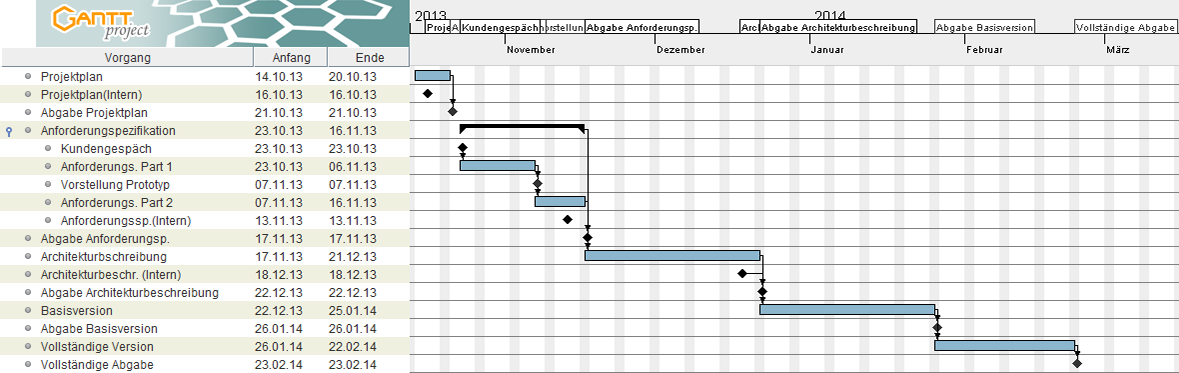
\includegraphics[scale=0.4]{Gantt-Ueberblick.png}
\label{Gantt-Ueberblick}
\end{figure}

\paragraph{Hinweise zu den Begriffen in den Tabellen:} \textit{Der Punkt 'Gesamtdauer' der jeweiligen Arbeitspakete ist der Zeitbereich zwischen dem Beginn und dem Ende einer bestimmten Aktivität. Der 'Aufwand' ist die tatsächlich aufgewendete Zeit, in der auch gearbeitet wurde. Somit kann die 'Gesamtdauer' häufig höher ausfallen, wenn sich bestimmte Aktivitäten z.B. über Feiertage hinziehen. Mit der 'Abhängigkeit' ist gemeint, ob das Arbeitspaket von anderen abhängig ist, also im Prinzip einen Vorgänger hat. Mit den 'Ressourcen' sind stets Akteure unserer Gruppe gemeint. Der Punkt 'Mindestanforderungen' beschreibt gewissermaßen das Minimalziel des Arbeitspakets (Minimalbedingung), die mindestens erfüllt werden muss, damit es fertig ist.}\\

\subsubsection{Projektplan}\label{aps}

In den folgenden Tabellen sind die Arbeitspakete des Abschnitts 'Projektplan' dargestellt. Grafisch sind diese in einem weiteren Gantt-Diagramm realisiert (Abbildung \ref{Gantt-Projektplan}). \\

\begin{figure}[htbp]
\caption{Gantt-Projektplan}
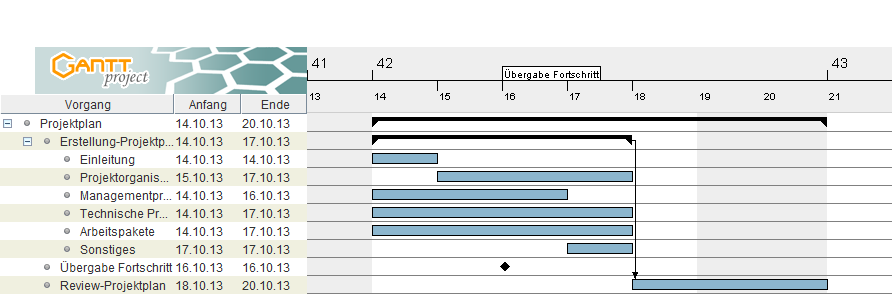
\includegraphics[scale=0.56]{Gantt-Projektplan.png}
\newline
\label{Gantt-Projektplan}
\end{figure}


\begin{tabular}{p{7.5cm}|p{7.5cm}}\toprule
\multicolumn{2}{c}{\textbf{\textit{A R B E I T S P A K E T \quad 1}}} \\ \toprule \hline
\textbf{Bezeichnung} & Gesamter Projektplan\\\hline
\multicolumn{2}{p{15cm}}{\textbf{Beschreibung:} \newline 
Anfertigung und Komplettierung des initalen Projektplans. Details erfolgen in den jeweiligen Unterpunkten.}  \\\hline
\textbf{Hauptverantwortlicher} & Patrick Damrow\\\hline
\textbf{Abhängigkeit} & -\\\hline
\textbf{Ressourcen} & -\\\hline
\textbf{Aufwand, Gesamtdauer} & \\\hline
\textbf{Beginn} & 14.10.2013 \\\hline
\textbf{Ende} & 20.10.2013\\\hline
\multicolumn{2}{p{15cm}}{\textbf{Mindestanforderungen: } \newline
Die Fertigstellung des initialen Projektplans ist erfolgt und wird durch das interne Gruppen-Review von allen Gruppenmitgliedern überprüft und abgesegnet (Qualitätssicherung).}  \\ \toprule
\end{tabular} \\\\

\begin{tabular}{p{7.5cm}|p{7.5cm}}\toprule
\multicolumn{2}{c}{\textbf{\textit{A R B E I T S P A K E T \quad 1.1}}} \\ \toprule \hline
\textbf{Bezeichnung} & Projektplanerstellung\\\hline
\multicolumn{2}{p{15cm}}{\textbf{Beschreibung:} \newline 
siehe Unterpunkte}  \\\hline
\textbf{Hauptverantwortlicher} & Tobias Dellert und Tim Ellhoff\\\hline
\textbf{Abhängigkeit} & -\\\hline
\textbf{Ressourcen} & -\\\hline
\textbf{Aufwand, Gesamtdauer} & \\\hline
\textbf{Beginn} & 16.10.2013 \\\hline
\textbf{Ende} & 17.10.2013\\\hline
\multicolumn{2}{p{15cm}}{\textbf{Mindestanforderungen: } \newline
Die Unterpunkte des Projektplans wurden abgearbeitet und der Projektplan kann im Gruppenreview überprüft werden.}  \\ \toprule
\end{tabular} \\\\

\begin{tabular}{p{7.5cm}|p{7.5cm}}\toprule
\multicolumn{2}{c}{\textbf{\textit{A R B E I T S P A K E T \quad 1.1.1}}} \\ \toprule \hline
\textbf{Bezeichnung} & Einleitung\\\hline
\multicolumn{2}{p{15cm}}{\textbf{Beschreibung:} \newline 
\textit{Erledigung des Projektplanteils:} Die Projektübersicht liefert die Ziele, Hauptarbeitsaktivitäten und -produkte, die Hauptmeilensteine und einen groben Zeitplan, die Erfassung der Ressourcen, die zur Verfügung stehenden Budgets sowie die Kontaktdaten des Kunden und Informationen über die Mitarbeiter am Projekt. Des Weiteren beinhaltet die Einleitung eine Übersicht der auszuliefernden  Produkte mit Terminangaben , sowie Informationen über die Evolution des Plans und die Festlegung von Definitionen bzw. Akronymen.}  \\\hline
\textbf{Hauptverantwortlicher} & Patrick Damrow\\\hline
\textbf{Abhängigkeit} & -\\\hline
\textbf{Ressourcen} & \begin{itemize}
\itemsep0pt
\item Patrick Damrow
\end{itemize} \\\hline
\textbf{Aufwand, Gesamtdauer} & \\\hline
\textbf{Beginn} & 16.10.2013 \\\hline
\textbf{Ende} & 17.10.2013\\\hline
\multicolumn{2}{p{15cm}}{\textbf{Mindestanforderungen: } \newline
Sobald der Projektplanteil fertig ist, kann er zum Gruppenreview weitergegeben werden. }  \\ \toprule
\end{tabular} \\\\

\begin{tabular}{p{7.5cm}|p{7.5cm}}\toprule
\multicolumn{2}{c}{\textbf{\textit{A R B E I T S P A K E T \quad 1.1.2}}} \\ \toprule \hline
\textbf{Bezeichnung} & Projektorganisation\\\hline
\multicolumn{2}{p{15cm}}{\textbf{Beschreibung:} \newline 
\textit{Erledigung des Projektplanteils:} In diesem Abschnitt wird das verwendete Prozessmodell beschrieben, die Organisationsstruktur festgelegt (insbes. Pflichten der Gruppenmitglieder, Kommunikationswege, wöchentliche Treffen usw.), Informationen zu den Organisationsschnittstellen wie Auftraggeber und Arbeitgeber gegeben und letztlich die Verantwortlichkeiten im Projekt festgelegt und unter den einzelnen Gruppenmitgliedern aufgeteilt.    }  \\\hline
\textbf{Hauptverantwortlicher} & Patrick Damrow\\\hline
\textbf{Abhängigkeit} & -\\\hline
\textbf{Ressourcen} & \begin{itemize}
\itemsep0pt
\item Patrick Damrow
\end{itemize} \\\hline
\textbf{Aufwand, Gesamtdauer} & \\\hline
\textbf{Beginn} & 16.10.2013 \\\hline
\textbf{Ende} & 16.10.2013\\\hline
\multicolumn{2}{p{15cm}}{\textbf{Mindestanforderungen: } \newline
Sobald der Projektplanteil fertig ist, kann er zum Gruppenreview weitergegeben werden. }  \\ \toprule
\end{tabular} \\\\

\begin{tabular}{p{7.5cm}|p{7.5cm}}\toprule
\multicolumn{2}{c}{\textbf{\textit{A R B E I T S P A K E T \quad 1.1.3}}} \\ \toprule \hline
\textbf{Bezeichnung} & Managementprozess\\\hline
\multicolumn{2}{p{15cm}}{\textbf{Beschreibung:} \newline 
\textit{Erledigung des Projektplanteils:} Im Managementprozess erfolgt die Festlegung der Managementprozesse (insbes. Ziele des Projekts), sowie die Einhaltung von gewissen Regeln im Punkt 'Annahmen', die eine Vereinbarung der Abhängigkeiten, an denen das Projekt unmittelbar geknüpft ist und die Erfassung von Einschränkungen, die berücksichtigt werden müssen, mit einschließt. Es folgen Angaben zum Risikomanagement (insbes. Ausfall bzw. Austritt von Gruppenmitgliedern, allgemeine Probleme etc.) , Maßnahmen zur Projektüberwachung sowie die Fixierung der Kompetenzen der Mitarbeiter im Projekt.  }  \\\hline
\textbf{Hauptverantwortlicher} & Daniel Pupat\\\hline
\textbf{Abhängigkeit} & -\\\hline
\textbf{Ressourcen} & \begin{itemize}
\itemsep0pt
\item Daniel Pupat
\end{itemize} \\\hline
\textbf{Aufwand, Gesamtdauer} & \\\hline
\textbf{Beginn} & 16.10.2013 \\\hline
\textbf{Ende} & 16.10.2013\\\hline
\multicolumn{2}{p{15cm}}{\textbf{Mindestanforderungen: } \newline
Sobald der Projektplanteil fertig ist, kann er zum Gruppenreview weitergegeben werden. }  \\ \toprule
\end{tabular} \\\\

\begin{tabular}{p{7.5cm}|p{7.5cm}}\toprule
\multicolumn{2}{c}{\textbf{\textit{A R B E I T S P A K E T \quad 1.1.4}}} \\ \toprule \hline
\textbf{Bezeichnung} & Technische Prozesse\\\hline
\multicolumn{2}{p{15cm}}{\textbf{Beschreibung:} \newline 
\textit{Erledigung des Projektplanteils:} In diesem Abschnitt erfolgt die Festlegung der Entwicklungsplattformen, -methoden und der verwendeten Programmiersprache, sowie eine Vereinbarung über die Eckpfeiler der im Laufe es Projekts abzugebenden Dokumentationen. Unterstützende Projektfunktionen wie die Ernennung von Phasenleitern und die Verwendung eines Versionskontrollsystems nebst Datensicherungen wird schließlich vereinbart. }  \\\hline
\textbf{Hauptverantwortlicher} & Sebastian Bredehöft \\\hline
\textbf{Abhängigkeit} & -\\\hline
\textbf{Ressourcen} & \begin{itemize}
\itemsep0pt
\item Sebastian Bredehöft
\end{itemize} \\\hline
\textbf{Aufwand, Gesamtdauer} & \\\hline
\textbf{Beginn} & 16.10.2013 \\\hline
\textbf{Ende} & 16.10.2013\\\hline
\multicolumn{2}{p{15cm}}{\textbf{Mindestanforderungen: } \newline
Sobald der Projektplanteil fertig ist, kann er zum Gruppenreview weitergegeben werden. }  \\ \toprule
\end{tabular} \\\\

\begin{tabular}{p{7.5cm}|p{7.5cm}}\toprule
\multicolumn{2}{c}{\textbf{\textit{A R B E I T S P A K E T \quad 1.1.5}}} \\ \toprule \hline
\textbf{Bezeichnung} & Arbeitspakete, Zeitplan u. Budget\\\hline
\multicolumn{2}{p{15cm}}{\textbf{Beschreibung:} \newline 
\textit{Erledigung des Projektplanteils:} In diesem Punkt werden die Arbeitspakete aller Projektphasen erarbeitet. Zunächst folgen gewisse Annahmen und Anmerkungen sowie Begrifferklärungen für die Arbeitspakete, bevor dann kleinschrittig die Arbeitspakete in tabellarischer und grafischer Form erfasst werden. Es folgen weitere Arbeitspakete für die Dokumentabgaben, Informationen und Vereinbarungen über Meetings innerhalb der Gruppe und der Festlegung des kritischen Pfads für das Projekt.}  \\\hline
\textbf{Hauptverantwortlicher} & Tobias Dellert, Tim Ellhoff \\\hline
\textbf{Abhängigkeit} & -\\\hline
\textbf{Ressourcen} & \begin{itemize}
\itemsep0pt
\item Tobias Dellert
\item Tim Ellhoff
\end{itemize} \\\hline
\textbf{Aufwand, Gesamtdauer} & \\\hline
\textbf{Beginn} & 16.10.2013 \\\hline
\textbf{Ende} & 17.10.2013\\\hline
\multicolumn{2}{p{15cm}}{\textbf{Mindestanforderungen: } \newline
Sobald der Projektplanteil fertig ist, kann er zum Gruppenreview weitergegeben werden. }  \\ \toprule
\end{tabular} \\\\

\begin{tabular}{p{7.5cm}|p{7.5cm}}\toprule
\multicolumn{2}{c}{\textbf{\textit{A R B E I T S P A K E T \quad 1.1.6}}} \\ \toprule \hline
\textbf{Bezeichnung} & Sonstige Elemente\\\hline
\multicolumn{2}{p{15cm}}{\textbf{Beschreibung:} \newline 
\textit{Erledigung des Projektplanteils:} Der Abschnitt 'Sonstiges' liefert Informationen über die Pläne für die Konvertierung von Daten, Management-, Ausbildungs- und Raum- und Installationspläne sowie den Plan über die letztendliche Abgabe bzw. Übergabe des Systems. }  \\\hline
\textbf{Hauptverantwortlicher} & Mohamadreza (Amir) Khostevan \\\hline
\textbf{Abhängigkeit} & -\\\hline
\textbf{Ressourcen} & \begin{itemize} 
\itemsep0pt
\item Mohamadreza (Amir) Khostevan
\end{itemize} \\\hline
\textbf{Aufwand, Gesamtdauer} & \\\hline
\textbf{Beginn} & 16.10.2013 \\\hline
\textbf{Ende} & 16.10.2013\\\hline
\multicolumn{2}{p{15cm}}{\textbf{Mindestanforderungen: } \newline
Sobald der Projektplanteil fertig ist, kann er zum Gruppenreview weitergegeben werden. }  \\ \toprule
\end{tabular} \\\\

\begin{tabular}{p{7.5cm}|p{7.5cm}}\toprule
\multicolumn{2}{c}{\textbf{\textit{A R B E I T S P A K E T \quad 1.2}}} \\ \toprule \hline
\textbf{Bezeichnung} & Gruppenreview des Projektplans\\\hline
\multicolumn{2}{p{15cm}}{\textbf{Beschreibung:} \newline 
Im internen Gruppenreview wird der fertige Projektplan diskutiert, ggf. verbessert bzw. noch geändert.}  \\\hline
\textbf{Hauptverantwortlicher} & Tobias Dellert, Tim Ellhoff \\\hline
\textbf{Abhängigkeit} & 1 Projektplan, 1.1 Projektplanerstellung\\\hline
\textbf{Ressourcen} & \begin{itemize}
\itemsep0pt
\item Tobias Dellert
\item Tim Ellhoff
\item Patrick Damrow
\item Sebastian Bredehöft
\item Daniel Pupat
\item Mohamadreza (Amir) Khostevan
\end{itemize} \\\hline
\textbf{Aufwand, Gesamtdauer} & \\\hline
\textbf{Beginn} & 19.10.2013 \\\hline
\textbf{Ende} & 19.10.2013\\\hline
\multicolumn{2}{p{15cm}}{\textbf{Mindestanforderungen: } \newline
Der Projektplan ist nun von allen Gruppenmitgliedern in einem Review noch einmal auf den Prüfstand gestellt worden und ist nun fertig. }  \\ \toprule
\end{tabular} \\\\

\subsubsection{Anforderungsspezifikation}\label{aps}

In den folgenden Tabellen sind die Arbeitspakete des Abschnitts 'Anforderungsspezifikation' dargestellt. Grafisch sind diese in einem weiteren Gantt-Diagramm realisiert\todo{Gantt-Diagramm+ Referenz}.

\begin{tabular}{p{7.5cm}|p{7.5cm}}\toprule
\multicolumn{2}{c}{\textbf{\textit{A R B E I T S P A K E T \quad 2}}} \\ \toprule \hline
\textbf{Bezeichnung} & Gesamte Anforderungsspezifikation\\\hline
\multicolumn{2}{p{15cm}}{\textbf{Beschreibung:} \newline 
Anfertigung und Komplettierung der Anforderungsspezifikation. Details erfolgen in den jeweiligen Unterpunkten.}  \\\hline
\textbf{Hauptverantwortlicher} & Daniel Pupat\\\hline
\textbf{Abhängigkeit} & -\\\hline
\textbf{Ressourcen} & -\\\hline
\textbf{Aufwand, Gesamtdauer} & \\\hline
\textbf{Beginn} & 21.10.2013 \\\hline
\textbf{Ende} & 17.11.2013\\\hline
\multicolumn{2}{p{15cm}}{\textbf{Mindestanforderungen: } \newline
Die Fertigstellung der Anforderungsspezifikation ist erfolgt.}  \\ \toprule
\end{tabular} \\\\

\begin{tabular}{p{7.5cm}|p{7.5cm}}\toprule
\multicolumn{2}{c}{\textbf{\textit{A R B E I T S P A K E T \quad 2.1}}} \\ \toprule \hline
\textbf{Bezeichnung} & Kundeninterview\\\hline
\multicolumn{2}{p{15cm}}{\textbf{Beschreibung:} \newline 
siehe Unterpunkte}  \\\hline
\textbf{Hauptverantwortlicher} & Tobias Dellert und Tim Ellhoff\\\hline
\textbf{Abhängigkeit} & -\\\hline
\textbf{Ressourcen} & -\\\hline
\textbf{Aufwand, Gesamtdauer} & \\\hline
\textbf{Beginn} & 21.10.2013 \\\hline
\textbf{Ende} & 30.10.2013\\\hline
\multicolumn{2}{p{15cm}}{\textbf{Mindestanforderungen: } \newline
Die Unterpunkte des Kundeninterviews wurden abgearbeitet. Der Ist-Zustand ist somit analysiert und dokumentiert.}  \\ \toprule
\end{tabular} \\\\

\begin{tabular}{p{7.5cm}|p{7.5cm}}\toprule
\multicolumn{2}{c}{\textbf{\textit{A R B E I T S P A K E T \quad 2.1.1}}} \\ \toprule \hline
\textbf{Bezeichnung} & Vorbereitung auf Kundeninterview\\\hline
\multicolumn{2}{p{15cm}}{\textbf{Beschreibung:} 
\newline 
Um ein effektives, aufschlussreiches Interview zu gewährleisten, ist eine konkrete Vorstellung der zu stellenden Fragen von Nöten. Ziel ist es, nach Möglichkeit alle Anforderungen und Wünsche des Kunden, sowohl die bewussten, als auch die unbewussten, herauszustellen. Dafür wird hier ein Fragenkatalog erstellt, der auf Kunden mit beliebigem Wissensstand über technische Details anwendbar ist.}  \\\hline
\textbf{Hauptverantwortlicher} & Tobias Dellert \\\hline
\textbf{Abhängigkeit} & -\\\hline
\textbf{Ressourcen} & \begin{itemize} 
\itemsep0pt
\item Tobias Dellert
\end{itemize} \\\hline
\textbf{Aufwand, Gesamtdauer} & \\\hline
\textbf{Beginn} & 21.10.2013 \\\hline
\textbf{Ende} & 21.10.2013\\\hline
\multicolumn{2}{p{15cm}}{\textbf{Mindestanforderungen: } \newline
Der entstehende Fragenkatalog muss weitestgehend alle Fragen enthalten, die für ein genaues Verständnis der Wünsche und Anforderungen des Kunden nötig sind. }  \\ \toprule
\end{tabular} \\\\

\begin{tabular}{p{7.5cm}|p{7.5cm}}\toprule
\multicolumn{2}{c}{\textbf{\textit{A R B E I T S P A K E T \quad 2.1.2}}} \\ \toprule \hline
\textbf{Bezeichnung} Kundeninterview\\\hline
\multicolumn{2}{p{15cm}}{\textbf{Beschreibung:} \newline 
Ein Gespräch mit dem oder den Kunden über bestehende Vorstellungen und Anforderungen, bezüglich der gewünschten Software. Ziel ist es, mithilfe des 
entworfenen Fragenkatalogs, sowohl bewusste Vorstellungen und Wünsche, wie auch die unbewussten 
herauszustellen, um den Kunden nach dem Kano-Modell zu begeistern. Die erworbenen Eindrücke und Vermutungen über die unbewussten Wünsche des oder der Kunden werden als Zusatz vorgeschlagen, um später unbezahlten Einsatz nach Einsetzen dieser Sonderfunktionen zu vermeiden. Kleinere Extras jedoch können vorerst im Hintergrund gehalten werden, um den Kunden bei der Präsentation des Endprodukts tatsächlich zu begeistern.  }  \\\hline
\textbf{Hauptverantwortlicher} & Tobias Dellert \\\hline
\textbf{Abhängigkeit} & -\\\hline
\textbf{Ressourcen} & \begin{itemize} 
\itemsep0pt
\item Tobias Dellert
\end{itemize} \\\hline
\textbf{Aufwand, Gesamtdauer} & \\\hline
\textbf{Beginn} & 23.10.2013 \\\hline
\textbf{Ende} & 23.10.2013\\\hline
\multicolumn{2}{p{15cm}}{\textbf{Mindestanforderungen: } \newline
Die erforderten Grundfunktionen wurden eindeutig 
herausgestellt und von Seiten des oder der Kunden bestätigt.  }  \\ \toprule
\end{tabular} \\\\

\begin{tabular}{p{7.5cm}|p{7.5cm}}\toprule
\multicolumn{2}{c}{\textbf{\textit{A R B E I T S P A K E T \quad 2.1.3}}} \\ \toprule \hline
\textbf{Bezeichnung} & Auswertung des  Kundeninterviews\\\hline
\multicolumn{2}{p{15cm}}{\textbf{Beschreibung:} \newline 
Die erhaltenen Auskünfte werde zusammengebracht und zu einem großem Bild aus Anforderungen zusammengefügt}  \\\hline
\textbf{Hauptverantwortlicher} & Daniel Pupat \\\hline
\textbf{Abhängigkeit} & -\\\hline
\textbf{Ressourcen} & \begin{itemize} 
\itemsep0pt
\item  Daniel Pupat
\end{itemize} \\\hline
\textbf{Aufwand, Gesamtdauer} & \\\hline
\textbf{Beginn} & 23.10.2013 \\\hline
\textbf{Ende} & 24.10.2013\\\hline
\multicolumn{2}{p{15cm}}{\textbf{Mindestanforderungen: } \newline
Das erhaltene Gesamtbild enthält alle gegebenen
Anforderungen, die nach dem Kundeninterview vom Kunden als Leistungsfaktoren angesehen werden.
 }  \\ \toprule
\end{tabular} \\\\

\begin{tabular}{p{7.5cm}|p{7.5cm}}\toprule
\multicolumn{2}{c}{\textbf{\textit{A R B E I T S P A K E T \quad 2.1.4}}} \\ \toprule \hline
\textbf{Bezeichnung} & Vergleich mit ähnlichen Softwaresystemen und Besuch in der SuUB Bremen\\\hline
\multicolumn{2}{p{15cm}}{\textbf{Beschreibung:} \newline 
Das entstandene Gesamtbild wird mit ähnlichen, bewährten Softwaresystemen verglichen. Deren Eigenheiten und daraus resultierende Vor- und Nachteile werden erschlossen und die Systeme als Ganzes bewertet. Zudem wird ein Besuch in der SuUB Bremen einen präzisierenden Einblick in die reale Verwaltungsarbeit der Mitarbeiter dieser SuUB ermöglichen, der mit dem Eindruck der Kundenbibliothek und dessen Möglichkeiten verglichen wird. Dies ist ein sehr sinnvoller Schritt, um ein erweitertes Weltbild der Verwaltungs- und Archivierungsarbeit zu erlangen und es auf unser Projekt anzuwenden.   }  \\\hline
\textbf{Hauptverantwortlicher} & Sebastian Bredehöft\\\hline
\textbf{Abhängigkeit} & -\\\hline
\textbf{Ressourcen} & \begin{itemize} 
\itemsep0pt
\item Sebastian Bredehöft
\item Tobias Dellert
\end{itemize} \\\hline
\textbf{Aufwand, Gesamtdauer} & \\\hline
\textbf{Beginn} & 31.10.2013 \\\hline
\textbf{Ende} & 01.11.2013\\\hline
\multicolumn{2}{p{15cm}}{\textbf{Mindestanforderungen: } \newline
Die Grundfunktion mindestens eines fremden, aber ähnlichen Softwaresystems wurden erfasst und mit unserem Gesamtbild von Anforderungen verglichen. }  \\ \toprule
\end{tabular} \\\\

\begin{tabular}{p{7.5cm}|p{7.5cm}}\toprule
\multicolumn{2}{c}{\textbf{\textit{A R B E I T S P A K E T \quad 2.2}}} \\ \toprule \hline
\textbf{Bezeichnung} & Kundenwünsche (Soll-Analyse)\\\hline
\multicolumn{2}{p{15cm}}{\textbf{Beschreibung:} \newline 
siehe Unterpunkte }  \\\hline
\textbf{Hauptverantwortlicher} & Sebastian Bredehöft\\\hline
\textbf{Abhängigkeit} & -\\\hline
\textbf{Ressourcen} & \begin{itemize} 
\itemsep0pt
\item Sebastian Bredehöft
\item Tobias Dellert
\end{itemize} \\\hline
\textbf{Aufwand, Gesamtdauer} & \\\hline
\textbf{Beginn} & 21.10.2013 \\\hline
\textbf{Ende} & 09.11.2013\\\hline
\multicolumn{2}{p{15cm}}{\textbf{Mindestanforderungen: } \newline
Die Kundenwünsche an das Produkt sind erfasst und hinreichend dokumentiert. }  \\ \toprule
\end{tabular} \\\\

\begin{tabular}{p{7.5cm}|p{7.5cm}}\toprule
\multicolumn{2}{c}{\textbf{\textit{A R B E I T S P A K E T \quad 2.2.1}}} \\ \toprule \hline
\textbf{Bezeichnung} & Herausstellen der Produktperspektiven\\\hline
\multicolumn{2}{p{15cm}}{\textbf{Beschreibung:} \newline 
Hier werden die gegebenen Rahmenbedingungen und Möglichkeiten analysiert, um die realistische Durchführung und dessen Aufwand zu erfassen. Beachtet und analysiert werden folgende Bereiche:\newline 

-Systemschnittstellen    \newline       
-Benutzerschnittstellen  \newline  
-Hardwareschnittstellen \newline        
-Softwareschnittstellen  \newline 
-Kommunikationsschnittstellen  \newline 
-Speicherbeschränkungen    \newline      
-Betriebsmodi     \newline              
-lokale Anpassungsfähigkeit

}  \\\hline
\textbf{Hauptverantwortlicher} & Tim Ellhoff \\\hline
\textbf{Abhängigkeit} & -\\\hline
\textbf{Ressourcen} & \begin{itemize} 
\itemsep0pt
\item Tim Ellhoff
\item Sebastian Bredehöft
\end{itemize} \\\hline
\textbf{Aufwand, Gesamtdauer} & \\\hline
\textbf{Beginn} & 01.11.2013 \\\hline
\textbf{Ende} & 02.11.2013\\\hline
\multicolumn{2}{p{15cm}}{\textbf{Mindestanforderungen: } \newline
Die in der Beschreibung aufgezählten Punkte können in der Anforderungsspezifikation eindeutig und exakt beschrieben werden. }  \\ \toprule
\end{tabular} \\\\

\begin{tabular}{p{7.5cm}|p{7.5cm}}\toprule
\multicolumn{2}{c}{\textbf{\textit{A R B E I T S P A K E T \quad 2.2.2}}} \\ \toprule \hline
\textbf{Bezeichnung} & Verschriftlichung der Rahmenbedingungen\\\hline
\multicolumn{2}{p{15cm}}{\textbf{Beschreibung:} \newline 
Es werden sowohl technische, als auch gesetzliche Rahmenbedingungen festgelegt. Zusätzlich sollen 
sicherheitskritische Aspekte durch genauere Spezifikationen der einzelnen Schnittstellen im vorigen Arbeitspaket 2.2.1
begutachtet werden. }  \\\hline
\textbf{Hauptverantwortlicher} & Patrick Damrow \\\hline
\textbf{Abhängigkeit} & 2.2.1 Herausstellen der Produktperspektiven \\\hline
\textbf{Ressourcen} & \begin{itemize} 
\itemsep0pt
\item Patrick Damrow
\end{itemize} \\\hline
\textbf{Aufwand, Gesamtdauer} & \\\hline
\textbf{Beginn} & 25.10.2013 \\\hline
\textbf{Ende} & 25.10.2013\\\hline
\multicolumn{2}{p{15cm}}{\textbf{Mindestanforderungen: } \newline
Die technischen und gesetzlichen Rahmenbedingungen sind eindeutig spezifiziert. Alle sicherheitskritischen Aspekte
wurden erfasst. }  \\ \toprule
\end{tabular} \\\\

\begin{tabular}{p{7.5cm}|p{7.5cm}}\toprule
\multicolumn{2}{c}{\textbf{\textit{A R B E I T S P A K E T \quad 2.2.3}}} \\ \toprule \hline
\textbf{Bezeichnung} & Auflistung von Anwendungsfällen\\\hline
\multicolumn{2}{p{15cm}}{\textbf{Beschreibung:} \newline 
Die einzelnen Anwendungsfälle werden hier aufgelistet und kurz beschrieben. Zum Beispiel: Einloggen, Nutzer oder Bibliothekar in das System einloggen.}  \\\hline
\textbf{Hauptverantwortlicher} & Mohamadreza (Amir) Khostevan \\\hline
\textbf{Abhängigkeit} & -\\\hline
\textbf{Ressourcen} & \begin{itemize} 
\itemsep0pt
\item Mohamadreza (Amir) Khostevan
\end{itemize} \\\hline
\textbf{Aufwand, Gesamtdauer} & \\\hline
\textbf{Beginn} & 25.10.2013 \\\hline
\textbf{Ende} & 25.10.2013\\\hline
\multicolumn{2}{p{15cm}}{\textbf{Mindestanforderungen: } \newline
Die Anwendungsfälle aller Grundfunktionen sind erfasst und kurz beschrieben. }  \\ \toprule
\end{tabular} \\\\

\begin{tabular}{p{7.5cm}|p{7.5cm}}\toprule
\multicolumn{2}{c}{\textbf{\textit{A R B E I T S P A K E T \quad 2.2.4}}} \\ \toprule \hline
\textbf{Bezeichnung} & Erstellung der Persona\\\hline
\multicolumn{2}{p{15cm}}{\textbf{Beschreibung:} \newline 
Sinn dieses Arbeitspakets ist es, einen vollständigen Einblick des für uns relevanten Ausschnitts der Realität zu erhalten, um damit in sich geschlossene Strukturen von den einzelnen Akteuren untereinander zu schaffen und damit einen verbesserten Überblick der möglichen Anwendungsfälle zu bekommen. Hierzu werden Benutzerklassen erstellt, die so gut wie möglich die unterschiedlichsten Charaktere, Umstände und Motive im Rahmen des Bibliotheksverwaltungsbereichs abdecken. }  \\\hline
\textbf{Hauptverantwortlicher} & Daniel Pupat \\\hline
\textbf{Abhängigkeit} & -\\\hline
\textbf{Ressourcen} & \begin{itemize} 
\itemsep0pt
\item Daniel Pupat
\end{itemize} \\\hline
\textbf{Aufwand, Gesamtdauer} & \\\hline
\textbf{Beginn} & 25.10.2013 \\\hline
\textbf{Ende} & 25.10.2013\\\hline
\multicolumn{2}{p{15cm}}{\textbf{Mindestanforderungen: } \newline
 Die entstandenen Persona sind umfassend und untereinander verschieden genug, um alle möglichen Anwendungsfälle in Bezug auf die erforderten Grundfunktionen der Software zu erhalten. }  \\ \toprule
\end{tabular} \\\\

\begin{tabular}{p{7.5cm}|p{7.5cm}}\toprule
\multicolumn{2}{c}{\textbf{\textit{A R B E I T S P A K E T \quad 2.2.5}}} \\ \toprule \hline
\textbf{Bezeichnung} & Überblick, sowie Ausblick in die Zukunft  \\\hline
\multicolumn{2}{p{15cm}}{\textbf{Beschreibung:} \newline 
Überblick der Abhängigkeiten von projekteigenen Faktoren untereinander, sowie ein Blick in die nahe Zukunft, was  Veränderungen und Erweiterungen sowohl im technischen und rechtlichen Bereich, sowie im Anwendungsumfeld der zu entwickelnden Software angeht. Die Anforderungen sollen entsprechend veränder- und anpassbar sein.}  \\\hline
\textbf{Hauptverantwortlicher} & Tim Ellhoff \\\hline
\textbf{Abhängigkeit} & -\\\hline
\textbf{Ressourcen} & \begin{itemize} 
\itemsep0pt
\item Tim Ellhoff
\end{itemize} \\\hline
\textbf{Aufwand, Gesamtdauer} & \\\hline
\textbf{Beginn} & 28.10.2013 \\\hline
\textbf{Ende} & 28.10.2013\\\hline
\multicolumn{2}{p{15cm}}{\textbf{Mindestanforderungen: } \newline
Die Abhängigkeit des Entwicklungs- und Erweiterungsprozess
von einzelnen pojekteigenen Faktoren wurden umfassend herausgestellt. Zu erwartende Veränderungen in der nahen Zukunft( sofern vorhanden ) wurden dokumentiert. }  \\ \toprule
\end{tabular} \\\\

\begin{tabular}{p{7.5cm}|p{7.5cm}}\toprule
\multicolumn{2}{c}{\textbf{\textit{A R B E I T S P A K E T \quad 2.3.1}}} \\ \toprule \hline
\textbf{Bezeichnung} & Datenmodell\\\hline
\multicolumn{2}{p{15cm}}{\textbf{Beschreibung:} \newline 
Das zu entwickelnde Datenmodell soll eine konzeptionelle Darstellung von dem Weltausschnitt in der Bibliothek, als UML-Diagramm, werden.}  \\\hline
\textbf{Hauptverantwortlicher} & Tobias Dellert \\\hline
\textbf{Abhängigkeit} & -\\\hline
\textbf{Ressourcen} & \begin{itemize} 
\itemsep0pt
\item Tobias Dellert
\end{itemize} \\\hline
\textbf{Aufwand, Gesamtdauer} & \\\hline
\textbf{Beginn} & 28.10.2013 \\\hline
\textbf{Ende} & 28.10.2013\\\hline
\multicolumn{2}{p{15cm}}{\textbf{Mindestanforderungen: } \newline
Die Informationen und deren Beziehungen sind dem Weltausschnitt entsprechend in das Datenmodell gesetzt und es lässt sich somit als Konzept für spätere Spezifizierungen benutzen. }  \\ \toprule
\end{tabular} \\\\

\begin{tabular}{p{7.5cm}|p{7.5cm}}\toprule
\multicolumn{2}{c}{\textbf{\textit{A R B E I T S P A K E T \quad 2.3.2.1}}} \\ \toprule \hline
\textbf{Bezeichnung} & Die genaueren Anwendungsfälle \\\hline
\multicolumn{2}{p{15cm}}{\textbf{Beschreibung:} \newline 
Die bereits aufgelisteten Anwendungsfälle werden mit den Personas und genaueren Beschreibungen ergänzt. Das Hineinversetzen in die unterschiedlichen Personas hilft die bisherige Funktionalität aus der Sicht der Mitarbeiter und späteren Kunden zu sehen. }  \\\hline
\textbf{Hauptverantwortlicher} & Sebastian Bredehöft \\\hline
\textbf{Abhängigkeit} & -\\\hline
\textbf{Ressourcen} & \begin{itemize} 
\itemsep0pt
\item Sebastian Bredehöft
\end{itemize} \\\hline
\textbf{Aufwand, Gesamtdauer} & \\\hline
\textbf{Beginn} & 29.10.2013 \\\hline
\textbf{Ende} & 29.10.2013\\\hline
\multicolumn{2}{p{15cm}}{\textbf{Mindestanforderungen: } \newline
Die Anwendungsfälle müssen insgesamt die ganze gewünschte Funktionalität der Software wiedergeben.  }  \\ \toprule
\end{tabular} \\\\

\begin{tabular}{p{7.5cm}|p{7.5cm}}\toprule
\multicolumn{2}{c}{\textbf{\textit{A R B E I T S P A K E T \quad 2.3.2.2}}} \\ \toprule \hline
\textbf{Bezeichnung} & Screenshots der Benutzeroberfläche\\\hline
\multicolumn{2}{p{15cm}}{\textbf{Beschreibung:} \newline 
Die Screenshots der Benutzeroberflächen werden benutzt, um die spezifischen Anwendungsfälle zu illustrieren. Dazu werden die Screenshots an de passenden Stellen beschriftet.}  \\\hline
\textbf{Hauptverantwortlicher} & Mohamadreza (Amir) Khostevan \\\hline
\textbf{Abhängigkeit} & -\\\hline
\textbf{Ressourcen} & \begin{itemize} 
\itemsep0pt
\item Mohamadreza (Amir) Khostevan
\end{itemize} \\\hline
\textbf{Aufwand, Gesamtdauer} & \\\hline
\textbf{Beginn} & 30.10.2013 \\\hline
\textbf{Ende} & 30.10.2013\\\hline
\multicolumn{2}{p{15cm}}{\textbf{Mindestanforderungen: } \newline
Alle Anwendungsfälle habe die ihnen zugehörigen Screenshots samt Beschriftung zugeteilt bekommen.}  \\ \toprule
\end{tabular} \\\\

\begin{tabular}{p{7.5cm}|p{7.5cm}}\toprule
\multicolumn{2}{c}{\textbf{\textit{A R B E I T S P A K E T \quad 2.2.3.3}}} \\ \toprule \hline
\textbf{Bezeichnung} & Anwendungs- und Sequenzdiagramme\\\hline
\multicolumn{2}{p{15cm}}{\textbf{Beschreibung:} \newline 
Die Anwendungsfälle werden passenderweise in Anwendungsdiagramme übertragen, wobei bei komplexeren Fällen 
zum Wohle der Übersicht auch Sequenzdiagramme hinzugezogen werden können. }  \\\hline
\textbf{Hauptverantwortlicher} & Patrick Damrow \\\hline
\textbf{Abhängigkeit} & -\\\hline
\textbf{Ressourcen} & \begin{itemize} 
\itemsep0pt
\item Patrick Damrow
\end{itemize} \\\hline
\textbf{Aufwand, Gesamtdauer} & \\\hline
\textbf{Beginn} & 01.11.2013 \\\hline
\textbf{Ende} & 01.11.2013\\\hline
\multicolumn{2}{p{15cm}}{\textbf{Mindestanforderungen: } \newline
Die Anwendungsfälle der Grundfunktionen sind in einem Anwendungsfalldiagramm dargestellt. }  \\ \toprule
\end{tabular} \\\\

\begin{tabular}{p{7.5cm}|p{7.5cm}}\toprule
\multicolumn{2}{c}{\textbf{\textit{A R B E I T S P A K E T \quad 2.3.3}}} \\ \toprule \hline
\textbf{Bezeichnung} & Aktionen\\\hline
\multicolumn{2}{p{15cm}}{\textbf{Beschreibung:} \newline 
Die bisher beschriebenen Anwendungsfälle werden noch genauer ausgeführt, sodass jede aufgelistete Aktion eine einzelne Nutzung einer beliebigen Funktion( Knopfdruck, Klick ins Textfeld ) der Software beschreibt.}  \\\hline
\textbf{Hauptverantwortlicher} & Mohamadreza (Amir) Khostevan \\\hline
\textbf{Abhängigkeit} & -\\\hline
\textbf{Ressourcen} & \begin{itemize} 
\itemsep0pt
\item Mohamadreza (Amir) Khostevan
\end{itemize} \\\hline
\textbf{Aufwand, Gesamtdauer} & \\\hline
\textbf{Beginn} & 16.10.2013 \\\hline
\textbf{Ende} & 16.10.2013\\\hline
\multicolumn{2}{p{15cm}}{\textbf{Mindestanforderungen: } \newline
Alle Anwendungsfälle sind in die kleinstmöglichen Aktionen aufgeteilt und geordnet. }  \\ \toprule
\end{tabular} \\\\

\begin{tabular}{p{7.5cm}|p{7.5cm}}\toprule
\multicolumn{2}{c}{\textbf{\textit{A R B E I T S P A K E T \quad 2.4}}} \\ \toprule \hline
\textbf{Bezeichnung} & Erstellung des GUI-Prototyps\\\hline
\multicolumn{2}{p{15cm}}{\textbf{Beschreibung:} \newline 
Hier wird erstmals eine Benutzeroberfläche auf Basis des Kundeninterviews und der einfachen Auflistung aller Anwendungsfälle geschaffen und dem Kunden vorgestellt.}  \\\hline
\textbf{Hauptverantwortlicher} & Tobias Dellert \\\hline
\textbf{Abhängigkeit} & -\\\hline
\textbf{Ressourcen} & \begin{itemize} 
\itemsep0pt
\item Tobias Dellert
\end{itemize} \\\hline
\textbf{Aufwand, Gesamtdauer} & \\\hline
\textbf{Beginn} & 06.11.2013 \\\hline
\textbf{Ende} & 06.11.2013\\\hline
\multicolumn{2}{p{15cm}}{\textbf{Mindestanforderungen: } \newline
Die Grundfunktionen müssen anhand des Prototyps  präsentierbar sein. }  \\ \toprule
\end{tabular} \\\\

\begin{tabular}{p{7.5cm}|p{7.5cm}}\toprule
\multicolumn{2}{c}{\textbf{\textit{A R B E I T S P A K E T \quad 2.4.1}}} \\ \toprule \hline
\textbf{Bezeichnung} & Prototyp-Vorstellung\\\hline
\multicolumn{2}{p{15cm}}{\textbf{Beschreibung:} \newline 
Dem Kundengespräch folgend, wird dem Kunden nun eine 
Benutzeroberfläche vorgestellt, welche abgesehen von den Leistungsfunktionen nach Möglichkeit bereits kleine Extras beinhalten soll, um den Kunden zu gewinnen. }  \\\hline
\textbf{Hauptverantwortlicher} & Mohamadreza (Amir) Khostevan \\\hline
\textbf{Abhängigkeit} & -\\\hline
\textbf{Ressourcen} & \begin{itemize} 
\itemsep0pt
\item Mohamadreza (Amir) Khostevan
\end{itemize} \\\hline
\textbf{Aufwand, Gesamtdauer} & \\\hline
\textbf{Beginn} & 06.11.2013 \\\hline
\textbf{Ende} & 06.11.2013\\\hline
\multicolumn{2}{p{15cm}}{\textbf{Mindestanforderungen: } \newline
Mit dem Prototyp lassen sich die Leistungsfaktoren präsentieren }  \\ \toprule
\end{tabular} \\\\

\begin{tabular}{p{7.5cm}|p{7.5cm}}\toprule
\multicolumn{2}{c}{\textbf{\textit{A R B E I T S P A K E T \quad 2.5}}} \\ \toprule \hline
\textbf{Bezeichnung} & Anforderungsspezifikation komplettieren\\\hline
\multicolumn{2}{p{15cm}}{\textbf{Beschreibung:} \newline 
Maßnahme, um Ergebnisse zusammenzufassen und zu korrigieren. Zusätzlich wird noch besonders Wert auf langfristige Schwachstellen des momentanen Ist-Zustand gelegt.    }  \\\hline
\textbf{Hauptverantwortlicher} & Daniel Pupat \\\hline
\textbf{Abhängigkeit} & -\\\hline
\textbf{Ressourcen} & \begin{itemize} 
\itemsep0pt
\item Daniel Pupat
\item Tim Ellhoff
\item Tobias Dellert
\end{itemize} \\\hline
\textbf{Aufwand, Gesamtdauer} & \\\hline
\textbf{Beginn} & 06.11.2013 \\\hline
\textbf{Ende} & 06.11.2013\\\hline
\multicolumn{2}{p{15cm}}{\textbf{Mindestanforderungen: } \newline
Sobald der Projektplanteil fertig ist, kann er zum Gruppenreview weitergegeben werden. }  \\ \toprule
\end{tabular} \\\\

\begin{tabular}{p{7.5cm}|p{7.5cm}}\toprule
\multicolumn{2}{c}{\textbf{\textit{A R B E I T S P A K E T \quad 2.6}}} \\ \toprule \hline
\textbf{Bezeichnung} & Angebot für den Kunden\\\hline
\multicolumn{2}{p{15cm}}{\textbf{Beschreibung:} \newline 
Angebot für den Kunden inkl. Kostenaufwand wird erstellt. }  \\\hline
\textbf{Hauptverantwortlicher} & Mohamadreza (Amir) Khostevan \\\hline
\textbf{Abhängigkeit} & -\\\hline
\textbf{Ressourcen} & \begin{itemize} 
\itemsep0pt
\item Mohamadreza (Amir) Khostevan
\item Patrick Damrow
\item Sebastian Bredehöft
\end{itemize} \\\hline
\textbf{Aufwand, Gesamtdauer} & \\\hline
\textbf{Beginn} & 14.11.2013 \\\hline
\textbf{Ende} & 15.11.2013\\\hline
\multicolumn{2}{p{15cm}}{\textbf{Mindestanforderungen: } \newline
Das Angebot für den Kunden ist hinreichend erstellt und kann nun dem Gruppenreview übergeben werden. }  \\ \toprule
\end{tabular} \\\\

\begin{tabular}{p{7.5cm}|p{7.5cm}}\toprule
\multicolumn{2}{c}{\textbf{\textit{A R B E I T S P A K E T \quad 2.7}}} \\ \toprule \hline
\textbf{Bezeichnung} & Gruppeninternes Review u. Finalisierung Anforderungsspezifikation\\\hline
\multicolumn{2}{p{15cm}}{\textbf{Beschreibung:} \newline 
Das Dokument wird in der Gruppe auf den Prüfstand gestellt und ggf. noch verändert bzw. verbessert.}  \\\hline
\textbf{Hauptverantwortlicher} & Tobias Dellert \\\hline
\textbf{Abhängigkeit} & 2.5 Anforderungsspezifikation komplettieren\\\hline
\textbf{Ressourcen} & \begin{itemize} 
\itemsep0pt
\item Tobias Dellert
\item Sebastian Bredehöft
\item Daniel Pupat
\item Patrick Damrow
\item Tim Ellhoff
\item Mohamadreza (Amir) Khostevan
\end{itemize} \\\hline
\textbf{Aufwand, Gesamtdauer} & \\\hline
\textbf{Beginn} & 15.11.2013 \\\hline
\textbf{Ende} & 15.11.2013\\\hline
\multicolumn{2}{p{15cm}}{\textbf{Mindestanforderungen: } \newline
Nach der Diskussion in der Gruppe wurde das Dokument optimiert und fertiggestellt. }  \\ \toprule
\end{tabular} \\\\

\begin{tabular}{p{7.5cm}|p{7.5cm}}\toprule
\multicolumn{2}{c}{\textbf{\textit{A R B E I T S P A K E T \quad 2.8}}} \\ \toprule \hline
\textbf{Bezeichnung} & Gruppeninternes Review u. Finalisierung Angebot\\\hline
\multicolumn{2}{p{15cm}}{\textbf{Beschreibung:} \newline 
Das Angebot für den Kunden wird in der Gruppe auf den Prüfstand gestellt und ggf. noch verändert bzw. verbessert.}  \\\hline
\textbf{Hauptverantwortlicher} & Tobias Dellert \\\hline
\textbf{Abhängigkeit} & 2.6 Angebot für den Kunden\\\hline
\textbf{Ressourcen} & \begin{itemize} 
\itemsep0pt
\item Tobias Dellert
\item Sebastian Bredehöft
\item Daniel Pupat
\item Patrick Damrow
\item Tim Ellhoff
\item Mohamadreza (Amir) Khostevan
\end{itemize} \\\hline
\textbf{Aufwand, Gesamtdauer} & \\\hline
\textbf{Beginn} & 15.11.2013 \\\hline
\textbf{Ende} & 15.11.2013\\\hline
\multicolumn{2}{p{15cm}}{\textbf{Mindestanforderungen: } \newline
Nach der Diskussion in der Gruppe wurde das Angebot optimiert und fertiggestellt. }  \\ \toprule
\end{tabular} \\\\

\subsubsection{Architekturbeschreibung}\label{aps}

\paragraph{Hinweis:} \textit{Der folgende Abschnitt sowie die darin enthaltenen Arbeitspakete sind zu diesem Zeitpunkt des Projekts noch nicht vollständig. Es handelt sich vielmehr um eine grobe Planung.}\\

In den folgenden Tabellen sind die Arbeitspakete des Abschnitts 'Architekturbeschreibung' dargestellt. Grafisch sind diese in einem weiteren Gantt-Diagramm realisiert\todo{Gantt-Diagramm+ Referenz}.

\begin{tabular}{p{7.5cm}|p{7.5cm}}\toprule
\multicolumn{2}{c}{\textbf{\textit{A R B E I T S P A K E T \quad 3}}} \\ \toprule \hline
\textbf{Bezeichnung} & Gesamte Architekturbeschreibung\\\hline
\multicolumn{2}{p{15cm}}{\textbf{Beschreibung:} \newline 
siehe Unterpunkte}  \\\hline
\textbf{Hauptverantwortlicher} & Tim Ellhoff \\\hline
\textbf{Abhängigkeit} & 2. Gesamte Anforderungsspezifikation\\\hline
\textbf{Ressourcen} & -
\\\hline
\textbf{Aufwand, Gesamtdauer} & \\\hline
\textbf{Beginn} & 18.11.2013 \\\hline
\textbf{Ende} & 22.12.2013\\\hline
\multicolumn{2}{p{15cm}}{\textbf{Mindestanforderungen: } \newline
Komplettierung der gesamten Architekturbeschreibung. }  \\ \toprule
\end{tabular} \\\\

\begin{tabular}{p{7.5cm}|p{7.5cm}}\toprule
\multicolumn{2}{c}{\textbf{\textit{A R B E I T S P A K E T \quad 3.1}}} \\ \toprule \hline
\textbf{Bezeichnung} & Globale Analyse\\\hline
\multicolumn{2}{p{15cm}}{\textbf{Beschreibung:} \newline 
Erkennen der Einflussfaktoren und Probleme, Entwicklung von Strategien.}  \\\hline
\textbf{Hauptverantwortlicher} & Tim Ellhoff \\\hline
\textbf{Abhängigkeit} & 2. Gesamte Anforderungsspezifikation\\\hline
\textbf{Ressourcen} & -
\\\hline
\textbf{Aufwand, Gesamtdauer} & \\\hline
\textbf{Beginn} & 18.11.2013 \\\hline
\textbf{Ende} & 09.12.2013\\\hline
\multicolumn{2}{p{15cm}}{\textbf{Mindestanforderungen: } \newline
Alle drei Punkte der globalen Analyse wurden bearbeitet. }  \\ \toprule
\end{tabular} \\\\

\begin{tabular}{p{7.5cm}|p{7.5cm}}\toprule
\multicolumn{2}{c}{\textbf{\textit{A R B E I T S P A K E T \quad 3.1.1}}} \\ \toprule \hline
\textbf{Bezeichnung} & Einflussfaktoren\\\hline
\multicolumn{2}{p{15cm}}{\textbf{Beschreibung:} \newline 
Erkennen der Einflussfaktoren (Flexibilität, Veränderlichkeit, Auswirkung).}  \\\hline
\textbf{Hauptverantwortlicher} & Tim Ellhoff \\\hline
\textbf{Abhängigkeit} & 2. Gesamte Anforderungsspezifikation\\\hline
\textbf{Ressourcen} & \begin{itemize} 
\itemsep0pt
\item Tim Ellhoff
\item Sebastian Bredehöft
\end{itemize} \\\hline
\textbf{Aufwand, Gesamtdauer} & \\\hline
\textbf{Beginn} & 18.11.2013 \\\hline
\textbf{Ende} & 18.11.2013\\\hline
\multicolumn{2}{p{15cm}}{\textbf{Mindestanforderungen: } \newline
Die Einflussfaktoren bezogen auf die Flexibilität, Veränderlichkeit und Auswirkungen wurden erkannt.}  \\ \toprule
\end{tabular} \\\\

\begin{tabular}{p{7.5cm}|p{7.5cm}}\toprule
\multicolumn{2}{c}{\textbf{\textit{A R B E I T S P A K E T \quad 3.1.2}}} \\ \toprule \hline
\textbf{Bezeichnung} & Probleme analysieren und Strategien entwickeln\\\hline
\multicolumn{2}{p{15cm}}{\textbf{Beschreibung:} \newline 
Es können sich aus den Einflussfaktoren neue Probleme ergeben. Diese müssen erfasst und Lösungsstrategien entwickelt werden.}  \\\hline
\textbf{Hauptverantwortlicher} & Daniel Pupat \\\hline
\textbf{Abhängigkeit} & 2. Gesamte Anforderungsspezifikation \\ 
& 3.1.1 Einflussfaktoren\\\hline
\textbf{Ressourcen} & \begin{itemize} 
\itemsep0pt
\item Daniel Pupat
\item Tobias Dellert
\end{itemize} \\\hline
\textbf{Aufwand, Gesamtdauer} & \\\hline
\textbf{Beginn} & 19.11.2013 \\\hline
\textbf{Ende} & 19.11.2013\\\hline
\multicolumn{2}{p{15cm}}{\textbf{Mindestanforderungen: } \newline
Probleme werden aufgeschrieben und Strategien daraus entwickelt.}  \\ \toprule
\end{tabular} \\\\

\begin{tabular}{p{7.5cm}|p{7.5cm}}\toprule
\multicolumn{2}{c}{\textbf{\textit{A R B E I T S P A K E T \quad 3.2}}} \\ \toprule \hline
\textbf{Bezeichnung} & Konzeptionelle Sicht\\\hline
\multicolumn{2}{p{15cm}}{\textbf{Beschreibung:} \newline 
Die konzeptionelle Sicht muss mittels einer UML visualisiert und außerdem verschriftlicht werden.}  \\\hline
\textbf{Hauptverantwortlicher} & Tim Ellhoff \\\hline
\textbf{Abhängigkeit} & 2. Gesamte Anforderungsspezifikation \\ 
& 3.1.2 Probleme analysieren und Strategien entwickeln\\\hline
\textbf{Ressourcen} & \begin{itemize} 
\itemsep0pt
\item Tim Ellhoff
\item Daniel Pupat
\item Tobias Dellert
\item Patrick Damrow
\item Sebastian Bredehöft
\item Mohamadreza (Amir) Khostevan
\end{itemize} \\\hline
\textbf{Aufwand, Gesamtdauer} & \\\hline
\textbf{Beginn} & 20.11.2013 \\\hline
\textbf{Ende} & 21.11.2013\\\hline
\multicolumn{2}{p{15cm}}{\textbf{Mindestanforderungen: } \newline
Erstellung der konzeptionellen Sicht als UML und als Text ist erfolgt.}  \\ \toprule
\end{tabular} \\\\

\begin{tabular}{p{7.5cm}|p{7.5cm}}\toprule
\multicolumn{2}{c}{\textbf{\textit{A R B E I T S P A K E T \quad 3.3}}} \\ \toprule \hline
\textbf{Bezeichnung} & Modulsicht\\\hline
\multicolumn{2}{p{15cm}}{\textbf{Beschreibung:} \newline 
Die Modulsicht muss mittels einer UML visualisiert und außerdem verschriftlicht werden.}  \\\hline
\textbf{Hauptverantwortlicher} & Tobias Dellert \\\hline
\textbf{Abhängigkeit} & 2. Gesamte Anforderungsspezifikation \\ 
& 3.2 Konzeptionelle Sicht\\\hline
\textbf{Ressourcen} & \begin{itemize} 
\itemsep0pt
\item Tobias Dellert
\item Daniel Pupat
\item Tim Ellhoff
\item Patrick Damrow
\item Sebastian Bredehöft
\item Mohamadreza (Amir) Khostevan
\end{itemize} \\\hline
\textbf{Aufwand, Gesamtdauer} & \\\hline
\textbf{Beginn} & 21.11.2013 \\\hline
\textbf{Ende} & 25.11.2013\\\hline
\multicolumn{2}{p{15cm}}{\textbf{Mindestanforderungen: } \newline
Erstellung der Modulsicht als UML und als Text ist erfolgt.}  \\ \toprule
\end{tabular} \\\\

\begin{tabular}{p{7.5cm}|p{7.5cm}}\toprule
\multicolumn{2}{c}{\textbf{\textit{A R B E I T S P A K E T \quad 3.4}}} \\ \toprule \hline
\textbf{Bezeichnung} & Datensicht\\\hline
\multicolumn{2}{p{15cm}}{\textbf{Beschreibung:} \newline 
Das Datenmodell aus der Anforderungsspezifikation muss weiterentwickelt werden. Dazu wird der Plan im Text beschrieben.}  \\\hline
\textbf{Hauptverantwortlicher} & Tobias Dellert \\\hline
\textbf{Abhängigkeit} & 2. Gesamte Anforderungsspezifikation \\\hline
\textbf{Ressourcen} & \begin{itemize} 
\itemsep0pt
\item Tobias Dellert
\item Daniel Pupat
\item Tim Ellhoff
\item Patrick Damrow
\item Sebastian Bredehöft
\item Mohamadreza (Amir) Khostevan
\end{itemize} \\\hline
\textbf{Aufwand, Gesamtdauer} & \\\hline
\textbf{Beginn} & 25.11.2013 \\\hline
\textbf{Ende} & 01.12.2013\\\hline
\multicolumn{2}{p{15cm}}{\textbf{Mindestanforderungen: } \newline
Das Datenmodell ist weiterentwickelt worden. Plan ist beschrieben.}  \\ \toprule
\end{tabular} \\\\

\begin{tabular}{p{7.5cm}|p{7.5cm}}\toprule
\multicolumn{2}{c}{\textbf{\textit{A R B E I T S P A K E T \quad 3.5}}} \\ \toprule \hline
\textbf{Bezeichnung} & Ausführungssicht\\\hline
\multicolumn{2}{p{15cm}}{\textbf{Beschreibung:} \newline 
Die Ausführungssicht der Architektur wird grafisch oder textuell beschrieben.}  \\\hline
\textbf{Hauptverantwortlicher} & Tobias Dellert \\\hline
\textbf{Abhängigkeit} & 2. Gesamte Anforderungsspezifikation \\
& 3.3 Modulsicht \\\hline
\textbf{Ressourcen} & \begin{itemize} 
\itemsep0pt
\item Tobias Dellert
\item Daniel Pupat
\item Tim Ellhoff
\item Patrick Damrow
\item Sebastian Bredehöft
\item Mohamadreza (Amir) Khostevan
\end{itemize} \\\hline
\textbf{Aufwand, Gesamtdauer} & \\\hline
\textbf{Beginn} & 27.11.2013 \\\hline
\textbf{Ende} & 28.11.2013\\\hline
\multicolumn{2}{p{15cm}}{\textbf{Mindestanforderungen: } \newline
Gesamte Ausführungssicht ist beschrieben.}  \\ \toprule
\end{tabular} \\\\

\begin{tabular}{p{7.5cm}|p{7.5cm}}\toprule
\multicolumn{2}{c}{\textbf{\textit{A R B E I T S P A K E T \quad 3.6}}} \\ \toprule \hline
\textbf{Bezeichnung} & Zusammenhänge zw. Anwendungsfällen und Architektur\\\hline
\multicolumn{2}{p{15cm}}{\textbf{Beschreibung:} \newline 
Mithilfe von UML-Sequenzdiagrammen müssen die Zusammenhänge zwischen Anwendungsfällen und Architektur visualisiert werden. }  \\\hline
\textbf{Hauptverantwortlicher} & Tobias Dellert \\\hline
\textbf{Abhängigkeit} & 2. Gesamte Anforderungsspezifikation \\
& 3.3 Modulsicht \\\hline
\textbf{Ressourcen} & \begin{itemize} 
\itemsep0pt
\item Tobias Dellert
\item Daniel Pupat
\item Tim Ellhoff
\item Patrick Damrow
\item Sebastian Bredehöft
\item Mohamadreza (Amir) Khostevan
\end{itemize} \\\hline
\textbf{Aufwand, Gesamtdauer} & \\\hline
\textbf{Beginn} & 02.12.2013 \\\hline
\textbf{Ende} & 09.12.2013\\\hline
\multicolumn{2}{p{15cm}}{\textbf{Mindestanforderungen: } \newline
Zusammenhänge zwischen Anwendungsfällen und Architektur sind hinreichend beschrieben und mittels UML-Sequenzdiagrammen veranschaulicht.}  \\ \toprule
\end{tabular} \\\\

\begin{tabular}{p{7.5cm}|p{7.5cm}}\toprule
\multicolumn{2}{c}{\textbf{\textit{A R B E I T S P A K E T \quad 3.7}}} \\ \toprule \hline
\textbf{Bezeichnung} & Evolution\\\hline
\multicolumn{2}{p{15cm}}{\textbf{Beschreibung:} \newline 
Ggf. müssen Evolutionen (bzw. allgemein Änderungen) erfasst und beschrieben werden.}  \\\hline
\textbf{Hauptverantwortlicher} & Tobias Dellert \\\hline
\textbf{Abhängigkeit} & 2. Gesamte Anforderungsspezifikation \\
& 3.2 Konzeptionelle Sicht \\
& 3.3 Modulsicht \\
& 3.4 Datensicht \\
& 3.5 Ausführungssicht \\\hline
\textbf{Ressourcen} & \begin{itemize} 
\itemsep0pt
\item Tobias Dellert
\item Daniel Pupat
\end{itemize} \\\hline
\textbf{Aufwand, Gesamtdauer} & \\\hline
\textbf{Beginn} & 12.12.2013 \\\hline
\textbf{Ende} & 16.12.2013\\\hline
\multicolumn{2}{p{15cm}}{\textbf{Mindestanforderungen: } \newline
Veränderungen wurden hinreichend analysiert und beschrieben.}  \\ \toprule
\end{tabular} \\\\

\subsubsection{Implementierung}\label{aps}

\paragraph{Hinweis:} \textit{Der folgende Abschnitt sowie die darin enthaltenen Arbeitspakete sind zu diesem Zeitpunkt des Projekts noch nicht vollständig. Es handelt sich vielmehr um eine grobe Planung.}\\

In den folgenden Tabellen sind die Arbeitspakete des Abschnitts 'Implementierung' dargestellt. Grafisch sind diese in einem weiteren Gantt-Diagramm realisiert\todo{Gantt-Diagramm+ Referenz}.

\subsubsection{Test}\label{aps}

\paragraph{Hinweis:} \textit{Der folgende Abschnitt sowie die darin enthaltenen Arbeitspakete sind zu diesem Zeitpunkt des Projekts noch nicht vollständig. Es handelt sich vielmehr um eine grobe Planung.}\\

In den folgenden Tabellen sind die Arbeitspakete des Abschnitts 'Test' dargestellt. Grafisch sind diese in einem weiteren Gantt-Diagramm realisiert\todo{Gantt-Diagramm+ Referenz}.


\subsubsection{Dokumentabgaben}\label{aps}

\subsubsection{Sonstiges}\label{aps}

\subsubsection{Meetings}\label{aps}

\subsubsection{Kritischer Pfad}\label{aps}

%%%%%%%%%%%%%%%%%%%%%%%%%%%%%%%%%%%%%%%%%%%%%%%%%%%%%%%%%%%%%%%%%%%%%%%%
\section{Sonstige Elemente (Amir)}
ENTFÄLLT
\subsection{Pläne für die Konvertierung von Daten}
ENTFÄLLT

\subsection{Managementpläne für Unterauftragsnehmer}
ENTFÄLLT
{\em Wenn Fremdbibliotheken benutzt werden\dots}

\subsection{Ausbildungspläne}
ENTFÄLLT
{\em Hierunter fallen z.B. auch interne Schulungen, die Ihr
  durchführen wollt.}

\subsection{Raumpläne}
ENTFÄLLT
\dots

\subsection{Installationspläne}
ENTFÄLLT
\dots

\subsection{Pläne für die Übergabe des Systems}
ENTFÄLLT
\dots


\end{document}
